%%%%%%%%%%%%%%%%%%%%%%%%%%%%%%%%%%%%%%%%%%%%%%%%%%%%%%%%%%%%%%%%%%%%
%% I, the copyright holder of this work, release this of into the
%% public domain. This applies worldwide. In some countries this may
%% not be legally possible; if so: I grant anyone the right to use
%% this work for any purpose, without any conditions, unless such
%% conditions are required by law.
%%%%%%%%%%%%%%%%%%%%%%%%%%%%%%%%%%%%%%%%%%%%%%%%%%%%%%%%%%%%%%%%%%%%

\documentclass[
  print, %% This option enables the default options for the
           %% digital version of a document. Replace with `printed`
           %% to enable the default options for the printed version
           %% of a document.
  Table,   %% Causes the coloring of tables. Replace with `notable`
           %% to restore plain tables.
  nolof,     %% `lof` Prints the List of Figures. Replace with `nolof` to
           %% hide the List of Figures.
  nolot,     %% `lot` Prints the List of Tables. Replace with `nolot` to
           %% hide the List of Tables.
  %draft, %TODO remove, place final instead
  11pt, % TODO disscus this
  oneside  %% twoside for print
  %% More options are listed in the user guide at
  %% <http://mirrors.ctan.org/macros/latex/contrib/fithesis/guide/mu/fi.pdf>.
]{fithesis3}
%% The following section sets up the locales used in the thesis.
\usepackage[resetfonts]{cmap} %% We need to load the a T2A font encoding
%\usepackage[utf8]{inputenc}
\usepackage[T1]{fontenc}  % T2a commented %% to use the Cyrillic fonts with Russian texts.
\usepackage[
  main=english, %% By using `czech` or `slovak` as the main locale
                %% instead of `english`, you can typeset the thesis
                %% in either Czech or Slovak, respectively.
  english, czech %german, russian, slovak %% The additional keys allow
]{babel}        %% foreign texts to be typeset as follows:
%%
%%   \begin{otherlanguage}{german}  ... \end{otherlanguage}
%%   \begin{otherlanguage}{russian} ... \end{otherlanguage}
%%   \begin{otherlanguage}{czech}   ... \end{otherlanguage}
%%   \begin{otherlanguage}{slovak}  ... \end{otherlanguage}
%%
%% For non-Latin scripts, it may be necessary to load additional
%% fonts:
%\usepackage{paratype}
%\def\textrussian#1{{\usefont{T2A}{PTSerif-TLF}{m}{rm}#1}}

%%
%% The following section sets up the metadata of the thesis.
\thesissetup{
    date          = \the\year/\the\month/\the\day,
    university    = mu,
    faculty       = fi,
    type          = mgr,
    author        = Karel Kubíček,
    gender        = m,
    advisor       = {RNDr. Petr Švenda, Ph.D.},
    title         = {Optimisation heuristics in randomness testing},
    TeXtitle      = {Optimisation heuristics in randomness testing},
    keywords      = {randomness testing, cryptoanalysis, block functions, stream functions, hash functions, problem optimization, metaheuristics},
    TeXkeywords   = {randomness testing, cryptoanalysis, block functions, stream functions, hash functions, problem optimization, metaheuristics},
}

\thesislong{abstract}{%
Statistical testing of randomness is one of the automated ways of cryptoanalysis of cryptoprimitives. While traditional statistical batteries use fixed tests, research tool EACirc developed at Faculty of Informatics, Masaryk University design the tests dynamically to the analysed data. Its goal is to distinguish tested data from random data. The tool internally utilises simple heuristic based on hill climbing. This thesis researches other metaheuristics and their potential application in EACirc tool, as well as application of classification models as artificial neural networks.\\\\%
%
The thesis has following contributions:
\begin{itemize}
    \item Development of a testbed of 16 well-known cryptographic functions with necessary tools for direct comparison of various tools tested on same data. The tool as the dataset are published, and we tested all related work on the data.
    \item Extension of EACirc tool with three new metaheuristics. One of them outperforms all others with success rate, and it also provides a further advantage of more practical cryptanalysis.
    \item Proof of concept implementation of an artificial neural network for binary data together with a literature review of this area. However, the performance of the neural network is unsatisfactory, being able to detect only very strongly biased data.
\end{itemize}
}

\thesislong{thanks}{%todo: metacentrum?
I would like to thank members of CRoCS laboratory for a friendly environment with productive seasons and joyful fun and relaxation topics. From those, I thank EACirc team members, who consulted and criticised the topics presented in this thesis. Especially I thank Petr for supervising me with his never-ending enthusiasm for science at all.

I apologise to my friends, who deserved more of my presence, but they still kept me at least a bit social. I am very grateful to my girlfriend Marta, who never left me being normal and bored by the work, as well as having any unused free time.

Most of all I owe to my parents, who always stand behind me. You always sensed the moments, when I need you and you surprised me with nice support. I am proud of having you, thanks.
}
%% The following section sets up the bibliography.
\usepackage{csquotes}
\usepackage[              %% When typesetting the bibliography, the
  backend=biber,          %% `numeric` style will be used for the
  style=numeric,          %% entries and the `numeric-comp` style
  citestyle=numeric-comp, %% for the references to the entries. The
  sorting=none,           %% entries will be sorted in cite order.
  sortlocale=auto         %% For more unformation about the available
]{biblatex}               %% `style`s and `citestyles`, see:
%% <http://mirrors.ctan.org/macros/latex/contrib/biblatex/doc/biblatex.pdf>.
\addbibresource{thesis.bib} %% The bibliograpic database within
                          %% the file `example.bib` will be used.
\usepackage{makeidx}      %% The `makeidx` package contains
\makeindex                %% helper commands for index typesetting.
%% These additional packages are used within the document:
\usepackage{paralist}
\usepackage{amsmath}
\usepackage{amsthm}
\usepackage{amsfonts}
\usepackage{url}
\usepackage{menukeys}

% cref, has to be loaded after hyperref
\usepackage{hyperref}
\usepackage{cleveref}
% for long equation wrap
\usepackage{wrapfig}
% figure captions
\usepackage{caption}
% subcaption for 2 figures in one
\usepackage{subcaption}

% tables
\usepackage{tabularx}
% colored cells (cellcolor)
\usepackage{colortbl}

% my colours
\usepackage{xcolor}

%% My own inputs:
% enabling new fonts support (nicer)
\usepackage{lmodern}
% better typeset of line ends and so (nicer)
\usepackage{microtype}
% code
\usepackage{minted}

\usepackage{tikz}
\usetikzlibrary{shapes,arrows,positioning}
\usetikzlibrary{decorations.pathreplacing}

% package to make bullet list nicer
\usepackage{enumitem}
\setitemize{noitemsep,topsep=3pt,parsep=3pt,partopsep=3pt}

% intendation
\usepackage{parskip}

% my own progress commands
\newcommand{\todo}[1]{TODO: \textit{#1}}
\newcommand{\rewrite}[1]{rewrite: \textit{#1}}
\newcommand{\reread}[1]{reread: \textbf{#1}}

% table colours
\newcommand{\fd}{\cellcolor{red!13}}
\newcommand{\fn}{\cellcolor{green!13}}

% make captions italic
\usepackage[format=plain,
            font=it]{caption}
% rotate figures
\usepackage{rotating}

% Lubo's hack for margins
\newcommand{\lmar}{3cm}
\newcommand{\rmar}{3cm}
\usepackage[top=2.8cm, left=\lmar, right=\rmar, bottom=3cm]{geometry}
\def\changemargin#1#2{\list{}{\rightmargin#2\leftmargin#1}\item[]}
\let\endchangemargin=\endlist{}


\begin{document}

% English indentation, vertical, not horizontal
\setlength{\parskip}{5pt}
\setlength{\parindent}{0pt}

%% We will define several mathematical sectioning commands.
%\newtheorem{theorem}{Theorem}[section] %% The numbering of theorems
                               %% will be reset after each section.
%\newtheorem{lemma}[theorem]{Lemma}     %% The numbering of lemmas
%\newtheorem{corr}[theorem]{Corrolary}  %% and corrolaries will
                                %% share the counter with theorems.
%\theoremstyle{definition}
%\newtheorem{definition}{Definition}
%\theoremstyle{remark}
%\newtheorem*{remark}{Remark}

\chapter{Introduction}
\label{chap:introduction}

Cryptography is a field of computer science, used daily by all Internet users. Users connecting to HTTPS websites are using asymmetric cryptography to generate a symmetric key for encryption of the following communication. For such use-case, as well as various others, are used cryptographic primitives as public-key encryption functions, hash functions, block functions and stream functions. Current research of cryptoprimitives has a nontrivial goal. Design and develop algorithms, such that can hold against unknown threats as long as possible. Therefore cryptographers follow the standardised approach in cryptoprimitives development to ensure quality by a lengthy process of preparation, comparison and testing.

\section{Cryptoprimitives selection process}
\label{sec:crypto-sel-proc}

A standardisation committee reacts on inquiry for new or updated cryptoprimitive by issuing a competition for it. For example competitions during last 20 years were AES, which called for a symmetric block cipher, eSTREAM, for new stream ciphers, SHA-3 for hash function and CAESAR for authenticated ciphers. Those competitions last usually around five years. The first phase is collecting proposals, which are filtered in the second phase to the gradual selection of the winner candidate in the third. The winning solution became standard, and the developers will use it usually for at least ten years. For example, Data Encryption Standard was standardised in 1976, and Triple-DES modification surpassed it as a standard in 1999. Final successor Advanced Encryption Standard came in 2002, and it remains functional until today (2017).

\section{Cryptoanalysis}
\label{sec:cryptoanalysis}

During the second phase, proposals are analysed by cryptoanalysts. While proposing own design is possible for both skilled teams and almost cryptography beginners, the analysis is demanding process that needs both skill and time.

Cryptanalysis is expensive work, as the required cryptoanalyst skills are demanding. It consumes a significant amount of time to reject even proposals vulnerable to known threats. Therefore, a software tool capable of rejecting vulnerable proposals can save cryptoanalyst's time. Moreover, the cryptanalyst can use the tool for quicker dive into the candidates' specifications. Such tool can, for example, identify optional parts and show weak or even threat parts of the proposed function.

\subsection[Cryptorimitives properties]{Overview of expected properties of cryptorimitives}
\label{subsec:crypto-prop}

Field of the analysis, which is this thesis aiming for, are hash functions, block ciphers and stream ciphers (further referred as functions). There are several properties, formulated as a minimal set of conditions for these functions which has to be satisfied. If the function does not meet some property, it is considered weak, while satisfaction of all of the properties does not imply nonvulnerable function. Some of the properties are following.

Irreversibility without the encryption key: from given ciphertext, the attacker is not able to reconstruct any bit of plaintext with a probability higher than 50\,\%. If the probability were over 50\,\%, the ciphertext would reveal some information about the plaintext.

Strict avalanche criterion: every bit flip of plaintext changes around 50\,\% of output bits. Not satisfying this would allow an attacker to start with plaintext of zeroes and continuously modify single bits to get closer to given ciphertext.

Oracle, semantic security: even though plaintext usually does not look like a random data, the ciphertext have to look so. If the output were distinguishable from random data, it would reveal information about the plaintext. This property is tested in our tool EACirc. However, the previous properties are tested as well, yet not directly.

\section{Cryptoanalysis automisation}
\label{sec:cryptoanalysis-automisation}



\subsection[Optimization problem for a cryptoprimitive]{Building an optimization problem from property of cryptoprimitives}
\label{subsec:opti-crypto}


\section{Statistical testing}
\label{sec:stat-testing}

% The introduction to statistical testing in cryptography is deeply discussed in~\cite[Section~5.4]{menezes1996handbook} and brief and readable introduction presented Emil Simion in~\cite{simion2015relevance}.

Testing of randomness is a common area of statistics research. Thus statisticians have developed a rigorous theory of probability, and they also produced practical tools, that can test randomness. These tools are used even in cryptography to analyse function for properties from the previous section.

\subsection{Statistical batteries}
\label{subsec:stat-batt}

% The full list of the statistical batteries and their brief description is in \cref{chap:relatwork}.

The statistical battery is a set of simple tests, which are analysing simple properties of the binary stream. For example, a monobit test counts an amount of zeros and ones in the input data, which should be similar in the case of the uniform stream. The tests can analyse the stream for patterns, which should not be present in random data.

The design of the tests accords to some statistical property. As the theory behind the statistical test is complex, the development of the test is difficult. The test set is fixed, so they cannot adapt to the input. The main advantage of EACirc is an ability to adapt to tested data. The tool itself learns on given data, and after this learning process, the output is randomness test for this specific type of data.

Best known statistical batteries are (chronologically by time of development) NIST STS, Diehard and Dieharder and TestU01. While NIST STS is already completely surpassed by its successors, statisticians still consider it as a golden standard of statistical testing. The EACirc performs better than NIST STS, is comparable with Dieharder and currently perform worse than TestU01. The ultimate goal of implementation of metaheuristics would be surpassing Dieharder and compete with TestU01.

\subsection{EACirc}
\label{subsec:eacirc}

\section{EACirc computation loop}
\label{sec:eac-comp}

\section{EACirc's potential}
\label{sec:eac-potential}

\subsection{Individual representation}
\label{subsec:eac-indiv-repres}

\subsubsection{\textbf{Circuit}}
\label{subsubsec:eac-indiv-repres-circuit}

\subsubsection{\textbf{Polynomials}}
\label{subsubsec:eac-indiv-repres-poly}

\subsection{Speed-up of computation}
\label{subsec:eac-speedup}

\subsection{Evaluation}
\label{subsec:eac-eval}

\subsection{Learning process}
\label{subsec:eac-learning}

% supervised learning (everywhere in this thesis)

\section{Problem optimisation}
\label{sec:prob-opt}

\subsection{Metaheuristics}
\label{subsec:prob-opt-meta}

A computational problem is a task to find a feasible solution for given question. An optimisation problem is a task to find the feasible solution, which satisfies the criteria best. Usually, we formulate fitness function to compare how well are the criteria met. A heuristic is a problem specific technique for finding some an approximative solution, where exact techniques fail. Finally, the metaheuristic is technique abstracted from the problem so that it can be used for various optimisation problems.

Metaheuristics are applicable for optimisation problems if a programmer can provide three crucial parts. First is an instance of solution for the problem (despite the quality). Second is a function to vary the solution, called neighbourhood function. Third and usually the most important is the fitness function, which measures the quality of the solution. Metaheuristic uses these parts to follow the landscape of the problem, and they try to find better solutions during the time.

The main advantage of metaheuristics is that they are well known, compared together in many studies (see 849 references in \cite{talbi2009metaheuristics}) that also provided tips for the implementation.

\chapter{Current approaches in problem optimization}
\label{chap:optimisation}

The number of candidate solutions inspected simultaneously splits metaheuristics into two categories: single-solution based metaheuristics and population-based metaheuristics.

The main advantage of having multiple concurrent solutions is handling population diversity. Diversity can help avoid ending in local optima and together with other techniques can produce better individuals faster. However, maintaining the diversity of the population is difficult, if the fitness does not increase continuously. When an individual has a unique feature, which increases its fitness, it is going to be quickly spread in next generations, suppressing other promising, but not yet so well performing other individuals.

The initial version of EACirc tended to use the advantages of the genetic programming, which is a population-based metaheuristic. Encoding the candidate solutions as a simulated electronic circuit allowed operations for mutation and crossover. Together with fitness evaluation was the optimisation process specified and used on cryptographic data, it was capable of distinguishing weak sources from truly random data~\cite{svenda2013towards}.

However, this approach was very complex and not enough understood. The sexual crossover did not have a sound implementation for the circuits. Besides, the expectation about the diversity of the population was not analysed. Also the interpretation of the results difficult. The following solution proposed in \cite{sys2014constructing} simplified the interpretation by using the population of only one individual. This solution allowed statistical postprocessing of fitness values and together with categories evaluator surpassed the previous approach in all tests~\cite{sys2014constructing}. Althout the project still used genetics library, by usage of single individual, the used metaheuristic became iterated local search.

EACirc 4.0 simplified and optimised the computations by substituting GALib -- a genetic algorithm library by a custom implementation of the iterated local search. This work analyses the problem and tries other metaheuristics to answer the question if iterated local search is the best approach.

\section{Single-solution metaheuristics}
\label{sec:opt-single-sol}

\Cref{fig:opt-single-sol-overview} shows the classification of the improved variants of local search metaheuristics by authors of ParadisEO library.

\begin{figure}[H]
    \centering
    \footnotesize{
    \begin{tikzpicture}[->,>=stealth',level/.style={sibling distance = 7cm/#1,
        level distance = 1.5cm}, every node/.style = {shape=rectangle, 
        draw=white, align=center}]]
      \node {Strategies for improving local search}
        child { node [xshift=3 cm] {Iterate with different\\solutions} 
            child { node {Multi-start\\local search} }
            child { node [xshift=-0.8 cm] {Iterative local\\search, GRASP} }
        }
        child { node {Change landscape\\of the problem}
            child { node [yshift=-1.2 cm, xshift=-0.6 cm] {Change of the objective function\\or the input data}
                child { node {Guided\\local\\search} }
                child { node {Noisy method} }
                child { node {Smoothing\\method} } }
            child { node [yshift=-1.2 cm, xshift=0.6 cm]  {Use different\\neighbourhoods}
                child { node {Variable\\neighbourhood\\search} }
            } 
        }
        child { node [xshift=-3 cm] {Accept non-improving\\neighbours} 
            child { node [xshift=0.8 cm] {Simulated\\annealing} }
            child { node [xshift=-0.8 cm] {Tabu\\search} }
        };
    \end{tikzpicture}
    }
    \caption{Single-solution metaheuristics as specialized version of local search. The source:~\cite[figure~2.24, p.~125]{talbi2009metaheuristics}.}
    \label{fig:opt-single-sol-overview}
\end{figure}

\subsection{Local search}
\label{subsec:opt-single-sol-ls}

Local search is the very basic approach in problem optimisation. The search begins with single candidate solution, and it applies changes to this solution, so it creates a neighbour candidate. Then the local search compares fitnesses of these two solutions and selects the better candidate to the next generation. The algorithm iterates this approach until 
it finds a satisfactory solution, or it ran the limited amount of iterations.

The algorithm can also be referred as hill-climbing, as we with acceptance of an improving solution, we step up in the fitness space. Therefore local search often finds only the sub-optimal solution -- a local optimum.

Escaping local optima is an important phenomenon, as fitness function landscape depends on tested data, or on the specific evaluation approach.

As EACirc is using an iterated version of local search, the application of local search would be straightforward. However, this would decrease the capabilities of EACirc do to omit of the learning process.

\subsection{Iterative local search}
\label{subsec:opt-single-sol-ils}

Iterative local search is and extension of local search. After defined amounts of iteration of basic local search, the tested data are changed. The computation on one set of data is called an \textit{epoch}, and the amount of iteration is called \textit{epoch length}.

During the epoch, the fitness progress is non-decreasing, however, after the end of each epoch, fitness is expected to drop. The final fitness has to be tested on a new dataset, which applies for every metaheuristic. Therefore, we distinguish between the learning dataset and the testing dataset.

The \textit{epoch length} is the crucial parameter of this metaheuristic. A short epoch length can be computationally more demanding due to higher data consumption, and the solution may not be able to learn anything on the data. Too long \textit{epoch} leads to \textit{overfitting}, a situation when the individual is learning a specific pattern of the current dataset over general patterns of all datasets. Martin Ukrop examined the overfitting process in EACirc in~\cite[chapter~7]{ukropBcThesis}.

The EACirc have used the iterated local search since~\cite{sys2014constructing}. Therefore it is used as a baseline for single solution metaheuristics tested in this work.

\subsection{GRASP}
\label{subsec:opt-single-sol-grasp}

The greedy randomised adaptive search procedure is splitting each iteration into two steps: a feasible solution construction by greedy algorithm and performing the local search using the generated solution.

We abandoned this metaheuristic as we did not found any greedy algorithm for circuit construction, such that would reflect tested data. Also, it does not fit the iterative process of learning in \textit{epochs}.

\subsection{Multi-start local search}
\label{subsec:opt-single-sol-msls}

Multi-start local search is another approach how to surpass local optimum to find the global optimum. The metaheuristic starts the computation with $k$ randomly generated individuals that are concurrently optimised by local search.

This parallelism could increase the usage of the testing data in EACirc. The disadvantage is a more difficult evaluation, as Ukrop stated in~\cite[chapter~5]{ukropBcThesis}. It is a question if we should evaluate the best, or the average, or random solution, or more solution simultaneously. Another possible advantage of multi-start local search can be parallelization of the computation. However, EACirc computation is already parallelized, neither on the level of single computation. Due to statistical interpretation, we have to repeat the computation process 1\,000 times.

We decided not to cover multi-start local search, as saving a small fraction of computation time for more complicated interpretation is a bad trade-off.

\subsection{Guided local search}
\label{subsec:opt-single-sol-gls}

Guided local search is metaheuristic based on dynamic changing of the fitness function. If the metaheuristic got stuck in local optima, guided local search would change the fitness function so the individual can follow climbing.

The EACirc computation can get trapped in a local optimum mainly in two cases:

\begin{enumerate}[noitemsep,topsep=3pt,parsep=3pt,partopsep=3pt]
    \item the individual got lucky to guess current test set, but it will not be successful in next \textit{epoch}, or
    \item the individual is already successful due to finding feature of the tested data, but it could not get better.
\end{enumerate}

We do not need to fix the first case, as such individual would be replaced in next \textit{epoch}. However, we can use guided local search to improve individual from the second case. Our alternative fitness function can be designed as the sum of our current fitness and e.g. the number of connectors. Such fitness would simplify the solution, which would help us with the interpretation of the last individual. Alternatively, we can use completely different fitness function.

We decided to implement guided local search in EACirc, as it also represents single-solution metaheuristics with a change of the objective function from \cref{fig:opt-single-sol-overview}.

\subsection{Noisy method}
\label{subsec:opt-single-sol-nois}

The noisy method is another metaheuristic, which changes the fitness space to escape local optima. It is done by adding random noise to the input data, as Talbi described in~\cite[section 2.9.2]{talbi2009metaheuristics}. At the beginning of the computation, the noise is the strongest, and it disappears during the computation, so the final \textit{epochs} can be evaluated on the original data.

In EACirc, our research goal is already distinguishing pseudo-random data from truly random data. An additional random noise in the input would probably lead to an even more complicated learning process. For example, the noise could flip a bit on a position, which is necessary for distinguishing between the data sources. Therefore was this method abandoned.

\subsection{Smoothing method}
\label{subsec:opt-single-sol-smooth}

Smoothing method is the another metaheuristic, which uses changes in fitness function to escape local optima. The method is based on smoothing the landscape of fitness function by computing a local average of all neighbours to given distance. If the fitness is overall increasing in one direction, but more zoomed observation shows small fluctuation, smoothing method smooths the fluctuation and allows locating the global optima.

\textit{Neigbours} in EACirc are defined as solutions obtained by mutation of the circuit. Available mutations are connecting or disconnecting a connector, or change of the Boolean function in the node. The neighbourhood of an individual in EACirc is enormous (over $2^{25}$ neighbours in the distance one for basic EACirc setup), this method would not be possible due to computational requirements.

\subsection{Variable neighbourhood search}
\label{subsec:opt-single-sol-vns}

Variable neighbourhood search also changes the landscape of the problem. However, it does not modify the fitness function or its interpretation, but it defines other methods for neighbour selection. If the computation stuck in local optima, the neighbourhood method is changed. Alternatively, the neighbourhood can be changed periodically. This method does not guarantee to escape from local optima, as all neighbourhoods can contain only worse solutions.

Specifying different neighbourhood in EACirc is hard. However, the method lead us to a different idea. EACirc is heading two mutually exclusive problems. We would like to have circuit connected sparsely for easier interpretation of the final solution. However, we also want to have the circuit's input and output nodes connected. We can solve the problems by reduction of the searched neighbourhood.

If we already have a successful solution, we can inspect only solutions with fewer connectors. In contrast, if the circuit is not connected (therefore the circuit's fitness is equal to zero), we can inspect only the individual with more connectors.

\subsection{Simulated annealing}
\label{subsec:opt-single-sol-sa}

Remaining two single-solution metaheuristics can accept non-improving neighbours. Short term acceptance of worse solution can lead to escape from local optima and finding global optima in whole computation.

Simulated annealing metaheuristic is inspired by the physical process of annealing in metallurgy. Annealing is an iterative process of heating the metal to increase the size of the crystals, which reduces the probability of a defect. During the process, the metal is heated to lower and lower temperatures.

Simulated annealing uses variable temperature, which describes the probability of acceptance of worse neighbour. This probability is decreasing during the computations, such that in the beginning, the likelihood of acceptance of worse solution is high, but at the end of the computation, only better solutions are accepted.

This metaheuristic is widely used, which was the reason for implementing it as a testing scenario for metaheuristics as a representation of the group of single solution metaheuristics that accepts non-improving solutions. Its implementation in EACirc does not require complex changes, only the specification of this method.

However, this method is not specified for the iterative approach with learning \textit{epochs}. Also, the acceptance of non-improving solution can lead to discarding a well-performing solution.

\subsection{Tabu search}
\label{subsec:opt-single-sol-tabu}

Like Simulated annealing, Tabu search can also accept non-improving solutions to escape from local optima. However, the decision whether to accept a non-improving solution is not based on probability, but on knowledge, if considered solution was visited. Therefore, Tabu search holds a memory of visited solutions, called \textit{tabu list}, and it would not use twice the same solution. This way, Tabu search avoids cycles during the optimisation process.

Application of Tabu search in EACirc has several issues. Firstly, how to store used individuals (memory usage may be a problem), which can be solved by storing only a hash of the solution. Secondly, the neighbourhood space of an individual is huge, as stated in \cref{subsec:opt-single-sol-smooth}. It is higher than the number of individuals tested during whole computation. Choosing twice the same solution is unlikely. Therefore we decided to try only Simulated annealing and leave the decision of Tabu search implementation on the result of Simulated annealing.

\section{Multi-solutions metaheuristics}
\label{sec:opt-multi-sol}

Multi-solutions metaheuristics are usually inspired by biological processes of some population. The group of evolutionary algorithms is inspired by the process of biological evolution, that process a population of species and forms better individuals. The ant colony optimisation and swarm intelligence algorithms are based on motion behaviour of a colony of selected species.

Multi-solutions metaheuristics are usually more complex than single-solution metaheuristics. The complexity shows on many layers.

\begin{itemize}
    \item The implementation usually requires many configurable parameters; therefore it is more prone to programming mistakes.
    \item The fine-tuning of these parameters can be sensitive to the selected problem.
    \item The algorithm needs more computational resources due to overhead with maintenance more complex method.
\end{itemize}

These disadvantages may be paid off. The population together may prevent the algorithm stuck in local optima, as long as the metaheuristic maintains well the diversity of the population. Another straightforward advantage is an application in similar process, which inspired the metaheuristic.

\subsection{Evolutionary algorithms}
\label{subsec:opt-multi-sol-ea}

Evolutionary algorithms are a group of multi-solution metaheuristics inspired by the natural selection in the evolution of the species. They are the most spread and studied population-based metaheuristic, in computer science since the 1980s. Evolutionary algorithms can be used to solve both continuous and discrete problems, and they are also used for both single- and multi-objective problems.

The computation is an iterative loop of three main steps, together denoted as a generation. The evolution starts with a random population of initial solutions.

\begin{description}
    \item[Selection of parents] from the population. Usually based on the fitness function with some randomization technique.
    \item[Reproduction to new offsprings] using mutation and crossover -- an algorithm for recombination of two parents. 
    \item[Population replacement] by offsprings. Here can be again used the evaluation by fitness. 
\end{description}

This iterative approach can by usage of well-selected fitness, mutation and crossover increase the quality of the individual. The algorithm can be stopped by the number of generations or by achieving target fitness.

During the 40 years, many variants of evolutionary algorithms emerged.

\begin{description}
    \item[Genetic algorithms] traditionally use bit representation of the individuals. It applies both mutation and crossover to create new individuals. The selection of new population from the offsprings is stochastic.
    \item[Evolutions strategies] are used in continuous optimisation, so the individuals are represented by real values. The main way of creation new offsprings is the mutation; the crossover is rarely used. They apply elitist selection to form a new population.
    \item[Evolutionary programming] is used in series prediction problems and continuous optimisation. It emphasises mutation and does not use recombination. The population is selected stochastically.
    \item[Genetic programming] evolves programs as solutions. They are usually expressed as a tree (like abstract syntax tree). Both mutation and crossover are applied. Even though genetic programming is the least studied approach of evolutionary algorithms, and it is computationally expensive, it is used in classification problems.
\end{description}

Randomness testing is a discrete optimisation problem; therefore we may apply genetic algorithms and genetic programming. Genetic algorithms were used in multiple works for analysis of bias in ciphertext from round reduced TEA and DES functions~\cite{twoRoundsTea,fourRoundsTea,fiveRoundsTea,song2007cryptanalysis,husein2007genetic}. On the other side, we found no successful work on the same topic using genetic programming.

The most important decisions for the well-working genetic algorithm are the individual representation and evaluation. The works on TEA~~\cite{twoRoundsTea,fourRoundsTea,fiveRoundsTea} represented the individual as a binary mask, which was applied to the plaintext and key to produce biased ciphertexts The bias was statistically evaluated, so it was used as the fitness. EACirc also formerly used genetic algorithms, and it represents the individual as simulated electric circuit (this may be close to the definition of genetic programming). The fitness corresponds to the deviation between analysed and reference data.

Other possible implementation using genetic algorithms may be for polynomial encoded tool BoolTest~\cite{sys2017detecting}, which is still in submission phase. The representation by a binary polynomial in algebraic form fits the proposed idea of genetic algorithms. Mutation can be a simple flip of a variable; the crossover can take some of the terms of each individual.

% the most studied spread multi-solution metaheuristic
% application in descrete and continuous problems. And also single objective and multiobjective
% inspired by natural selection and evolution of species
% multiple variations - explain the vocabulary (genetic algorithms, evolutions strategies, evolutionary programming, genetic programming)
% the main idea of genetic algorithms
    % selection of parents
    % reproduction
        % evaluation
    % replacement of the population by offsprings
    % repeat
% difficulties with management of the diversity

% intentionally skip the genotype and phenotype

\subsection{Ant colony optimization}
\label{subsec:opt-multi-sol-aco}

The ant colony optimisation is an instance of swarm intelligence metaheuristics. This metaheuristic imitates the cooperative behaviour of ants. Every ant has a simple goal of collecting food, and the common goal is to find shorted path between the food and the nest. The motion of the ants is coordinated by their smell and a pheromone.

\begin{itemize}
    \item Every ant spreads pheromone on its trail.
    \item Ant prefers to take a path with more pheromone.
    \item The pheromone evaporates over time.
\end{itemize}

The common application of ant colony optimisation is on shortest path algorithms. The literature states many applications in travelling salesman problem~\cite{dorigo1997ant, dorigo1997ant}. However, the metaheuristic can also be applied to combinatorial problems, as the problem representation can be encoded to the graph structure and the shorted path algorithm may solve them. An example of such application can be formula satisfiability problem (SAT)~\cite{moritz2010solving}.

The problems solvable by ant colony optimisation are usually problems, where the solution is constructed from \textit{building blocks}. The pheromone can be associated with the block and it can describe the probability of using the block in the final solution. Such problem instances are used in EACirc's polynomial representation.

We wanted to use ant colony optimisation on polynomials, however, we did not find a suitable library for \texttt{Python} or \texttt{C++}, such that would allow evaluation of whole constructed individual. Libraries like \texttt{ACO-Pants}~\cite{acoPants} specialise for pathfinding, where every edge have to be weighted, while we would need to evaluate the whole path.

\subsection{Scatter search}
\label{subsec:opt-multi-sol-scatter}
% multi-solution variation of tabu search?
% main idea:
%   1. hold diverse population (use tabu search for help)
%   2. get the best individuals in such population
%   3. split the population into smaller sets
%   4. combine the shared qualities of the individuals within the set, to get the ultimate individual with the core functionality
% population = reference set 10-20 candidates; subsets can be for example of size 2-4
% merge new candidates to the reference set and iteratively continue with the main steps
% the algorithm may stop by number of iterations or by leaving the reference set unchanged
% application in EACirc: we do not know, how to merge solutions

The scatter search method is highly utilising the combination of the individuals. The algorithm holds a population of the best so far inspected individuals called \textit{reference set}. Like every population-based metaheuristic, the diversity of the \textit{reference set} is crucial. Scatter search is an iterative algorithm, where one iteration consists of 4 steps.

\begin{enumerate}
    \item The \textit{reference set} is split to a subset of size 2 to 4 individuals.
    \item We combine the individuals of the subsets to create new candidate individuals.
    \item We run a single-solution metaheuristic to improve the candidate individuals.
    \item The \textit{reference set} incorporates the candidate individuals based on fitness.
\end{enumerate}

The main problem of application is the second step, where are solutions combined. We would have to develop a function, which combines multiple solutions and takes their shared properties. However, there is no guarantee that various advanced individuals share the same property. Also, the approach is similar to evolutionary algorithms. Therefore we did not test it.

\subsection{Other swarm intelligence methods}
\label{subsec:opt-multi-sol-si}

The swarm intelligence metaheuristics adopt a collective behaviour of decentralised and self-organized systems. Similarly to ant colony optimisation, the behaviour of the swarm can be used to solve optimisation problems. Usually, the best application is in problems that are close to the origin of the behaviour of the swarm. Therefore, the main application is in decentralised control of robots, droids and other artificial individuals.

The application issues for our problem are similar as for ant colony optimisation.

\section{Other methods}
\label{sec:opt-other}

There are various optimisation methods, which are not classified as single or multi solutions metaheuristics. However, those models or algorithms are still capable of learning of classification.

The classification is important in machine learning area. Therefore, the following models have developed advanced methods not only to the process of learning but also the interpretation of the results, detection of outliers, learning on a low amount of data or non-complete data. Because of these advantages, we decided to experiment with them.

These models and algorithms can be used for various goals. Two main are feature selection and classification. Our principal aim is the classification, while we expect, that the model itself will select the features. The model has to adapt to the data. Therefore we cannot make manual feature selection.

% what ML problem specification heads-to?
% ML is well studied, but the main problem is selection of the method, fine-tuning the parameters and setting up the features

\subsection{Artificial neural networks}
\label{subsec:opt-other-ann}

% Introduce the idea - look for some thesis using btw. ANN
%   inspired by Hebbian learning
%   backpropagation: Werbos 1975
%      gradient descent (optimisation method for backpropagation)
% Cite usage - find commonly cited papers, go trough them quickly
%   images
%   curves (signals)
%   text (selection of features)
% No-one tried to analyse binary data
%   feature selection is not straightforward, as it is specific to analysed data and we would have to learn even the process of feature selection.
%       EACirc: the circuit can be viewed as a feature selector, where the features are used afterwards for statistical testing (in the $\chi^{2}$ test)

The artificial neural networks (ANN) are classification optimisation method inspired by the process of learning of brain and neural system. The initial idea was inspired by the research of Donald Hebb~\cite{hebb49learning}, who described the neurones and the process of learning of living beings neural systems. The Hebbian learning arose several trivial nonsupervised learning methods. Further development came with the invention of backpropagation algorithm by Paul Werbos~\cite{werbos75beyondThesis}. The last rapid increase of usability of artificial neural networks came in 2006 with significant speed-up both of algorithm and its application on GPUs, which allowed deeper networks and more analysed data due to parallelization, leading to rapid progress in scalability and usability of artificial neural networks.
% deeper introduction to ANN can be found in book http://www.deeplearningbook.org

The artificial neural network consists of purpose specialised layers. The first layer is called visible layer, and its input is the data for classification. Then there may be many hidden layers, which sequentially process the output of previous layers. The data proceed to the last -- output layer, which decides the classification. Each layer consists of neurones. Each neurone takes as input the output from all neurones of previous layers, and weight for each connection multiplies these outputs. The output is processed by an activation function, which ensures normalisation of the output. There are many types of activation function, and each layer can use different activation function. The most used activation function is a sigmoid function, with input from real number and output is usually from the interval $(-1, 1)$ or $(0, 1)$.

%\todo{citations: }
The artificial neural networks were used to solve various problems in classification and pattern recognition. The most common are applications in image processing, signal processing, text data processing and in robotics and system control.

In cryptography, we have seen fewer applications of ANN. The main area of application of ANN in cryptography is authentication~\cite{li2001remote}, as it is a classification problem, where learning methods can bring speed-up traded off by approximation that allows errors.

Application in encryption is even rarer. For example, researchers from Google Brain showed an experiment where they let neural network develop encryption function for communication, while another neural network was intercepting the communication and attempting to decrypt it~\cite{abadi2016learning}. Preceding works~\cite{shihab2006backpropagation, volna2012cryptography} did not get such attention as Google's work, but they had a similar objective with simpler assumptions. However, all these works are far from application in cryptography. The only inspiration from them to our project is normalisation of binary data to floats, that was done by encoding zero as $-0.5$ and one as $+0.5$. We have found no further relevant application of ANN in the classification of binary data.

We would like to utilise the developed approach of learning in classification by ANN. However, the application of ANN in our scope is not straightforward. We do not know in advance, what are the features in the data. Therefore the network has to have the whole ciphertext as an input. We encode the binary input to floats (0 as $-0.5$ and 1 as $+0.5$) based on intuition supported by other works~\cite{abadi2016learning,shihab2006backpropagation}. We tried both fully connected network (where every node is connected to every node of previous layer or every input bit), and convolution network, where the first layer has only a limited local interval of inputs. 

% shihab2006backpropagation http://docsdrive.com/pdfs/sciencepublications/jcssp/2006/710-715.pdf
%   ANN develops decryption of basic Boolean blocks of permutation and 'doping.'
%   backpropagation, three layers (12-16-12), bits as -0.5, +0,5, linear activation
%   they claim better security than DES (due to large state space), but it is a bullshit

% li2001remote http://ieeexplore.ieee.org/stamp/stamp.jsp?arnumber=963786
%   multiserver multiuser authentication - users classified by ANN

% volna2012cryptography https://pdfs.semanticscholar.org/0860/8a61506de48da7e93320a5844b081801374a.pdf
%   ANN creates encryption algorithm (same as Google's paper), 6 bits blocks
%   network 6-6-6, sigmoid, nothing about bits representation
%   they are not cryptographers! Security by obscurity (the key is the weight of connectors in the network), again bullshit (OMG, they even do not meet semantics security!)

\subsection{Other statistical classification methods}
%https://en.wikipedia.org/wiki/Statistical_classification

% SVM
% kNN
% Decision trees (C4.5 algorithm https://en.wikipedia.org/wiki/C4.5_algorithm)
% Bayesian networks
% ...

There are several other models or algorithms of statistical classification. Those are for example support vector machine (SVM), decision tree with a C4.5 algorithm, $k$-nearest neighbours algorithm ($k$-NN), Bayes classifier and many others. Those methods usually rely on good feature selection, which we do not perform in our scenario. Therefore, the application of those models was not examined within this work, but they might be an interesting question for further works.

\chapter{Experiment methodology}
\label{chap:method}

The primary testing goal of EACirc is to assess randomness of ciphertext of cryptographic functions. As most of the cryptographic functions are in a scope of automated analysis semantic secure, EACirc can identify non-randomness only for reduced functions. The functions can be reduced in a number of rounds, by processing selected plaintexts, and by selecting only specific bits of the output. As the analysis of reduced versions of cryptographic functions is the main goal of the EACirc project, it is also selected as the testing scenario for comparison of analysed metaheuristics.

The approach for evaluation is \todo{briefly?} described in \cref{subsec:eacirc}. The tested data were produced from 16 different cryptographic functions. These functions are reduced by the number of rounds. We selected intervals of rounds based on EACirc reference capabilities, such that the EACirc is capable of distinguishing function reduced to $i$ rounds, but it is not able to distinguish $i+1$ rounds\footnote{Further is this round setting referred as "an edge".}. Usually we test also $i-1$ and $i+2$ rounds, for broader comparison of the results with state of the art of cryptoanalysis.

EACirc works as distinguisher between tested dataset (produced by the cryptographic function) and reference random data. Formerly we used quantum random number generator (QRNG) services as the source of this reference data. This have following disadvantages:

\begin{itemize}
    \item Need of having QRNG data for the computation.
    \item Potential of an error due to bad data. QRNG are not error less, for example, Quantis device we tested in our laboratory produced \href{http://rtt.ics.muni.cz/ViewResults/Experiment/1732/}{biased data}. Detection of such biases is common use-case of randomness testing.
\end{itemize}

Therefore we switched from QRNG to pseudo random number generator (PRNG) PCG32~\cite{pcgGen} as reference data. PCG32 is fast and computationally strong PRNG. We did experiment of comparison PCG32 with QRNG and we found no bias, as well as we retested old results using QRNG newly with PRNG and the results are the same. Hence, we believe build-in PRNG is a more secure and convenient option.

\section{Used data}
\label{sec:method-data}

Previous works on EACirc analysed candidates of cryptoprimitives competitions~\cite{estreamMgrThesis,sha3Thesis,ukropMgrThesis}. These works extended EACirc by many functions sharing the same interface. This approach was effective for broad analysis of the competition candidates, but it does not test well-known cryptographic functions like AES and DES.

Therefore, for the comparison with other randomness testing tools and other research papers on semantics security, we decided select new test set of cryptographic functions. We chose the finalist of competitions SHA-3 (BLAKE, Grostl, JH, Keccak and Skein) and eSTREAM (HC-128, Rabbit, Salsa20, SOSEMANUK and Grain), and above that, we implemented other block (AES, DES, 3-DES and TEA) and stream (RC4) functions.

\subsection{Reimplementation of stream handling in EACirc}
\label{subsec:method-data-streams}

The implementation of SHA-3 and eStream candidates in EACirc was called \todo{projects}. The projects were handling everything related to data generation, specifically IV, key and plaintext. Every project had its own implementation of counter plaintext generator, strict avalanche criterion generator and so on.

For the implementation of the new project for block ciphers, we decided to reimplement data generation in more variable and modifiable way. For this, we decided for data manipulation via streams, whose can be nested into each other. Each stream implements simple interface with constructor and function \texttt{next}, which returns next test vector. The stream is specified only by the output size of the test vector.

The purpose of stream is unification of all data manipulation in the whole project, independently on the used cryptographic function. All streams inherit from abstract class \texttt{stream} with minimalistic interface. The streams have to specify its \texttt{size} and they have to implement method \texttt{next()}, which returns next test vector. We have currently many types of streams in EACirc.

\begin{itemize}
    \item Data sources streams, that are used as an input to cryptographic functions or as reference data. Example of such streams are:
    \begin{itemize}
        \item input streams: true and false bits generators, counter and multiple variants of the strict avalanche criterion generator, and
        \item PRNG's PCG32 and Mersenne Twister. \todo{cite?}
    \end{itemize}
    \item Projects of cryptographic functions. Namely project eSTREAM and SHA-3.
    \item Postprocessing streams are applied to data from cryptographic functions for more advanced experiments. They allows us analysis of selected bits of the function.
\end{itemize}

The streams are completely configurable via \texttt{JSON} configuration file. As the streams can be nested, the structure is described as a \texttt{JSON} tree. This updates changed the structure of the configuration file, therefore the configuration files are not backwards compatible. Nevertheless, the configuration is described and showed on examples in the project's documentation~\cite{EACirc-wiki-streams}.

All these changes significantly simplified the codebase, unified many implementations of the same functionality and broadened the experiment capabilities of EACirc. Therefore it was the main feature for EACirc~4.1 release.

\subsection{Implementation of functions}
\label{subsec:method-data-funcs}

As the source of AES, DES and 3-DES implementations was used educative repository~\cite{cryptoFunc}. The author of this repository verifies the encryption to the test vectors to ensure correctly working implementation. The only modification of the code is a limitation of the functions in the number of rounds.

TEA implementation is based on Wikipedia code~\cite{teaWiki}, and it was already implemented in EACirc before. The implementation was simplified and reduced due to changes in the interface. It is also reduced to selected amount of rounds.

RC4 is also based on the educative repository~\cite{cryptoFunc}, but as RC4 has no round structure, therefore, the code is unchanged.

All these functions together with the new interface of new block project and test vectors processing algorithm were released in minor version EACirc 4.1.

\paragraph{Corrections and code review of SHA-3 and eSTREAM functions} was another part of streams update. Multiple cryptographic functions from previous implementation were incorrectly round-reduced.
\label{par:method-data-funcs-bugs}

\begin{itemize}
    \item SHA-3 Skein, eSTREAM Rabbit, SOSEMANUK and F-FCSR were not round-reduced, but their implementation uses iterative approach, so we reduced them.
    \item eSTREAM HC-128 stated in the project documentation and in header file, it can be round-reduced, but it had no effect in the core function at all.
    \item eSTREAM Salsa20 used wrong implicit number of rounds for default settings.
\end{itemize}

These bugfixes together with fix of improper configuration of eSTREAM project were one of two major reasons for releasing EACirc 4.2. All these fixes together with valid configurations are described in project documentation~\cite{EACirc-wiki-streams}.

\subsection{Data generator tool}
\label{subsec:method-data-generator}

For direct comparison of the tested methods, we need to analyse the same data. EACirc has build in generation of test vectors, to feed the computation, as is described in \cref{sec:method-data}. Therefore, we implemented side project from EACirc for production of data. We call it \textit{Generator} and it shares the source code of functions with EACirc.

The \textit{Generator} is fully configurable via \texttt{JSON} configuration file as EACirc. The structure of the file is reduced, as the configuration describes only generated data. So the \textit{Generator} inherits all the capabilities of streams, providing complex control on the data production. For simplification and automation, we also prepared script, that generates configuration files for most common settings, which allows simple execution by command line arguments. For even simpler acces to testing data, we generated 160~MB file for each basic setup for each widely-known cryptographic function (described in \cref{subsec:method-data-funcs}) reduced to wide interval of rounds. This dataset is publicly accessible \href{https://drive.google.com/drive/folders/0B5Z1zst5NzwXQmFKaXgxREJWNk0?usp=sharing}{online}.

We have ongoing plan of publication, which will crucially utilize the \textit{Generator}. It will be paper on comparison of statistical testing tools on wide variety of cryptographic data. The \textit{Generator} will be used as it unifies many different cryptographic functions and it can reduce the functions in number of rounds, or selection of specified bits. The \textit{Generator} has already all the necessary features, so we can start with writing of the paper when we select the conference, we are aiming for.

Important work for the generator was fixing the implementation bugs, described in previous~\cref{par:method-data-funcs-bugs}.


\section{Methodology for specific optimisation methods}
\label{sec:method-spec}

As the tested scenarios vary not only by optimisation method but by used tools as well, the methodology changes for given metaheuristics. The base of the experiment was used for single-solution metaheuristics, as they were implemented directly to the EACirc and they inherited the experiment environment of our tool.

For direct inter-method comparison, we need to use the same data for testing. Therefore, all used data are generated from the same implementation, described in \cref{subsec:method-data-funcs}. The cross-method comparison is still sensitive to the testing approach, therefore we describe it in detail in following sections.


\subsection{Single-solution methodology}
\label{subsec:method-spec-ss}

All single solution metaheuristics were implemented into EACirc, therefore they share the same computation and interpretation. The solution is represented as simulation of a circuit, described in the \cref{subsubsec:eac-indiv-repres-circuit}.

The main advantage of single-solution metaheuristics is their simplicity and straightforward interpretation. However, the overall interpretation of EACirc results became complex, as we work with randomness that needs to be evaluated statistically. The complex approach also leads to significantly better results. The statistical evaluation as well as distributed computation automation is described below.


\subsubsection{\textbf{Statistical evaluation}}
\label{subsubsec:method-spec-ss-stat}

The fitness of an individual is a $p$-value of two sample $\chi^{2}$ test, which tests, if the output bytes per source have same distribution. For a well-working individual on a weak source of data, the fitness is close to 1. As the quality of the individual decreases, the fitness decreases as well. However, completely random guess like coin tossing has the $p$-value uniformly distributed on the interval (0, 1).

As the $p$-values are uniformly distributed for random guess, getting high $p$-value can imply two cases. Either the $\chi^{2}$ test rejected the hypothesis and scored high confidential output, or the tested data, or in case of random guess, we were lucky and obtained high value from uniform ditribution on interval $(0, 1)$. Therefore, we avoid interpretation of a single $p$-value, we collect an $p$-value per every \textit{epoch}, and we process these $p$-values to Kolmogorov-Smirnov test. It analyses the uniformity of usually 300 $p$-values. This test is using critical value $\alpha = 1\,\%$, therefore it rejects the null hypothesis that tested data seems nonrandom in 1\,\% of runs. To avoid such case, we run the experiment with the same settings 1\,000 times and we analyse the rejection rate given as the amount of failed KS tests over 1000. If it is around 1\,\%, the data seem to be random, while in it is much higher, the experiment rejected randomness hypothesis of tested data.

This approach is vastly increasing the amount of data needed for the computation, as well as the overall run-time. This method is a trade-off for the success rate of EACirc, as different evaluators do not need statistical evaluation. Hence they need much fewer data; however, such evaluators are slightly worse based on the results from~\cite{svenda2013towards}.

When we consider basic setup for single-solution metaheuristics, EACirc consumes 4.8\,GB of ciphertext of tested function (\cref{fig:dataUsage}). The runtime of the experiment on MetaCentrum varies from 4 to 20 hours on a single core.

%http://tex.stackexchange.com/questions/57732/placing-figures-inside-a-two-column-document 3rd answer
\begin{figure*}[t]
    \begin{equation*}
        \begin{aligned}
    \Sigma = 1\,000 \;
             \frac{\textnormal{runs}}
                  {\textnormal{experiment}}
             \cdot
             \left(
             300 \;
             \frac{\textnormal{epochs}}
                  {\textnormal{run}}
             \cdot
             1\,000 \;
             \frac{\textnormal{vectors}}
                  {\textnormal{epoch}}
             \cdot
             16 \;
             \frac{\textnormal{bytes}}
                  {\textnormal{vector}}
             \right) \approx\\
             \approx 4.8 \textnormal{\,GiB per experiment}
        \end{aligned}
    \end{equation*}
    \caption{The amount of tested data analysed by EACirc for a single configuration of randomness testing experiment. A single run also evaluates randomness of the data, however the capability of EACirc decreases in such mode, and single result is prone to incorrect evaluation due to statistical error.}
    \label{fig:dataUsage}
\end{figure*}


\subsubsection{\textbf{Computation automisation}}
\label{subsubsec:method-spec-ss-auto}

As EACirc needs repeated computation on MetaCentrum grid infrastructure, the automation for binary deployment, computation distribution, aggregation of the results and their postprocessing are required.

The scripts are executed in few following steps.

\begin{enumerate}[noitemsep,topsep=3pt,parsep=3pt,partopsep=3pt]
 \item Firstly, a preprocessor creates necessary configuration files for the experiment.
 \item Secondly, MetaCentrum scripts distribute the computation among the grid infrastructure.
 \item Thirdly, after the computation finishes the postprocessor script aggregate the results. 
 \item Finally, the table generator script generates a human readable version of the results as well as database dump of the whole experiment. The whole process is showed in \cref{fig:scripts}.
\end{enumerate}

The EACirc project formelly used tool Oneclick created by Lubomír Obrátil~\cite{obratilBcThesis}. The Oneclick was a single tool for both preprocessing and postprocessing phase, and the run was parametrized. However, this approach was programmed for BOINC infrastracture and it is outdated for the MetaCentrum. The advantages of new scripts are: 

\begin{itemize}
    \item they are single purpose, easier to modify one without affecting other,
    \item they are written in bash (running scripts for MetaCentrum scheduler) and Python (processing), so they do not need to be compiled,
    \item they maintained up-to-date for the newest EACirc,
    \item they are faster, as MetaCentrum computation do not require formerly used redundancy procedures.
\end{itemize}

These scripts are expected to be modified by individual researchers for the needs of their experiments, so the scripts are stored in GitHub repository~\cite{eaUtils}, and users are supposed to fork them. The repository also contains \texttt{readme.md} file, with specifies the first steps with computations on MetaCentrum with these scripts. Every script then contains documentation in the code (concerning expected modifications for individual purposes), and when it is run without arguments, it prints out a help message.

\begin{figure}[H]
    \centering{}
    
\begin{changemargin}{-3cm}{-3cm}
    \centering{}
    \rotatebox{-90}{
    \scalebox{0.9}{
    \tikzstyle{block} = [draw, rectangle, minimum height=3em, minimum width=3em]
    \tikzstyle{el} = [draw, ellipse, minimum height=3em, minimum width=3em]
    \tikzstyle{cl} = [cloud, cloud puffs=10,cloud puff arc=120, minimum height=3em, minimum width=3em]
    \begin{tikzpicture}[>=stealth, auto, node distance=3cm, every text node part/.style={align=center}]
        \node [el] (e) [] {\bf{experiment idea}};
        \node [block] (pre) [below of = e,yshift=0.5cm] {\bf{preprocessor}};
        \node [block,text width=3.5cm] (run) [below of = pre,yshift=-0.5cm] {\vspace{0.1cm}{\bf runner scripts} \texttt{run\_experiment.sh} runs for every config file script \texttt{single\_job.sh}};
        \node [block] (eac) [below of = run] {\bf{EACirc}};
        \node [block] (pos) [below of = eac,yshift=0.6cm] {\bf{postprocessor}};
        \node [block] (gen) [below of = pos,yshift=0.6cm] {\bf{table generator}};
        \node [el] (res) [below of = gen,yshift=0.6cm] {\bf{readable results}};

        \draw [->] (e) -- node [right] {researcher modifies\\general setting} (pre);
        \draw [->] (pre) -- node [right] {produces config for\\all combinations\\of function and round} (run);
        \draw [->] (run) -- node [right] {distributes computations\\on MetaCentrum grid} (eac);
        \draw [->] (eac) -- node [right] {results are returned\\to the frontend server} (pos);
        \draw [->] (pos) -- node [right] {aggregates the results\\and computes the statistics} (gen);
        \draw [->] (gen) -- node [right] {generates human readable tables\\and dump the results} (res);
    \end{tikzpicture}
    }
    }
\end{changemargin}
    
    \caption{Execution of EACirc on MetaCentrum grid -- order and purpose of the scripts.}
    \label{fig:scripts}
\end{figure}

\paragraph{Preprocessor}

EACirc computation is based on a configuration file with specification and environment settings for particular experiment. As the test suite contains tens variations of parameters, it is necessary to automatize config file creation, so the user would not make a mistake during this process.

The scripts are written in Python and are maintained in variants per the scenario of tested functions.

\paragraph{Running scripts}

The scripts for distribution of computation among the MetaCentrum network are a result of Martin Ukrop's thesis~\cite{ukropMgrThesis}. They are continuously maintained in \texttt{EACirc-utils} repository~\cite{eaUtils} for current EACirc version.

As each experiment needs to be run multiple times for statistical evaluation, the scripts repeat the computation in a loop with different seeds usually for 1\,000 times. All runs are then collected by running scripts.

The current version of these scripts is also published on the GitHub~\cite{eaUtils}, and the forked repository is ready to run experiments in the usual way.

\paragraph{Postprocessor}

As the computations are repeated for statistical significance, the postprocessor script has to aggregate results from many produced files. It searches through output files and collects the results. Afterwards, it calculates an aggregated statistics of the experiment.

The output of the postprocessor is \texttt{JSON} dump of the results, whose are used both for human readable results generation and also storing the results for later usage.

\paragraph{Table generator}

The generator takes as an input the \texttt{JSON} dump of the results from the postprocessor. Currently, it only generates a \LaTeX table with highlighted results, but it can be extended for more complex manipulation with the results.

\subsubsection{\textbf{Goal specification}}
\label{subsubsec:method-spec-ss-goal}

\todo{Petr's comments are not corrected}

The ultimate goal of the experiments with metaheuristics is increasing detection capabilities of nonrandomness of tested datastream. For testing and measuring how a metaheuristic performs, we analyse swet of functions described in \cref{sec:method-data}. We increase the resolution of the comparison by testing cryptographic function reduced in number of rounds. However, reduction of the function to specific number of rounds is still a very steep, therefore the goal is hardly measurable on this scenario. The randomness of the data increases rapidly with the additional rounds of the cryptographic function. We would need functions with a low increase of entropy per round as a benchmark, but we did not observe such behaviour by any of the tested functions, nor our own design of benchmarking function do not behave that way~\cite{EACirc-lut}.

Less ambitious, but still useful goal can be an increase of the rejection rate of the null hypothesis per experiment. Rejecting only 10\,\% of runs lead to difficulties with the analysis of the output test. The higher is the rejection rate, the easier is the interpretation of found distinguisher. Also, if our rejection rate is close to critical value $\alpha$, then the higher rejection rate can overcome the edge value\footnote{For 1000 runs per experiment, this edge value is typically $2\cdot\alpha$. Such results can happen in less than 0.15\,\% of the experiments.} and we can reject the overall null hypothesis about the randomness of the source with higher confidentiality.

Another goal can be a decrease in the number of computations or the amount of used data. As we usually fix the epoch length to 100 iterations, the data usage and CPU time are directly related. Moreover, as the amount of used data is already high in this settings of EACirc, the time comparison is more valuable than consumed data comparison.

We can also analyse specific goals per metaheuristics. Both Variable neighbourhood search and Guided local search set a complementary target in simplification of the circuits for later analysis. This goal is harder to measure, so the analysis is done less rigorously.

The EACirc project is using adaptive learning. During the computation, the tested data are changing. We analysed over-learning of the individuals during the learning process, and the over-learning can be analysed as well. Therefore, decrease over-learning can be another goal for metaheuristics.

%\subsection{Multi-solutions methodology}
%\label{subsec:method-spec-ms}

\subsection{ANN methodology}
\label{subsubsec:method-spec-ms-aco}

% data
% evaluation -> amount of data
% scripts

The neural netowrk also classifies test vectors into 2 datasets -- the tested set and the reference set. Therefore, the implementation of takes as input 2 binary files -- a tested file and reference file. We generate these files with the \textit{Generator}, so we ensure consistency and comparability of the results within approaches. The results are concretely for the \href{https://drive.google.com/drive/folders/0B5Z1zst5NzwXQmFKaXgxREJWNk0?usp=sharing}{published dataset}.

The execution of neural network consist of training phase, where we iteratively provide different learning batches of data, and evaluation phase, where we use fresh data for final evaluation of ratio of correctly classified test vectors. The whole computation needs significantly less input data than EACirc, as is shown in \cref{fig:ann-dataUsage}.

\begin{figure*}[t]
    \begin{equation*}
        \begin{aligned}
    \Sigma = 
             100 \;
             \frac{\textnormal{epochs}}
                  {\textnormal{experiment}}
             \cdot
             25 \;
             \frac{\textnormal{vectors}}
                  {\textnormal{epoch}}
             \cdot
             16 \;
             \frac{\textnormal{bytes}}
                  {\textnormal{vector}}
             %\approx\\
             \approx {40 \textnormal{\,kB for learning +} \atop {40 \textnormal{\,kB for evaluation}}}
        \end{aligned}
    \end{equation*}
    \caption{The amount of data analysed by neural network for a single configuration of randomness testing experiment.}
    \label{fig:ann-dataUsage}
\end{figure*}

We prepared automation scripts for easier analysis of multiple files together. We have script for sequential execution of all the runs for all binary files in directory, which produces \texttt{JSON} results file. This file is afterwards proceed by script, which plots the learning progress and final correct classification ratio.


\chapter{Results}
\label{chap:res}

% TODO strange introduction, but we want this information somewhere
To verify any implementation, we perform sanity experiment comparing random data to random data. Such a test gives us measured expected output in case that selected approach can not distinguish two tested streams. Expected value of such experiment differs per methodology, and therefore we state it per every test scenario.

% SS methodology ref
\section{Single-solution metaheuristics}
\label{sec:res-ss}

%http://stattrek.com/online-calculator/binomial.aspx

Single solutions metaheuristics use evaluation described in \cref{subsubsec:method-spec-ss-stat}. Briefly it means, we execute EACirc 1\,000 times independently with same setting and we evaluate, how many of the runs rejected randomness hypothesis. Number of rejections divided by number of runs is called \textit{rejection ratio}. As we use significance level $\alpha=1\,\%$, the random-random experiment should reject randomness hypothesis on average in $1\,\%$ of the runs. As we would like to have better confidentiality in this sanity experiment, we perform not only 1\,000 runs for this settings, but 100\,000 runs. Confidentiality for such run can be computed from the binomial distribution. For example, \textit{rejection rate} higher or equal to $1.2\,\%$ for random-random experiment can occur with probability 4.787\,\% for 1\,000 runs, while the probability decreases to less than 0.001\,\% for 100\,000 runs. We include the measured rejection value to the first row of result tables. Further rows contain results of round-reduced cryptographical functions.

\Cref{table:res-usable-ils,table:res-usable-sa,table:res-usable-gls,table:res-usable-vns} summarise results of tested single-solution metaheuristics applied in EACirc. Every row of the table corresponds to one cryptographical function. The lower index after the name specifies EACirc default number of rounds, that we restrict the functions to. The columns with -1, 0, +1 and +2 denote offset to the number of rounds specified in the index. For example AES$_{3}$ was tested reduced to two rounds, three rounds as default and four rounds. Five rounds were not tested, which is denoted by a dash in the cell. The number in cell represents the \textit{rejection ratio}. For indistinguishable data, values around measured ratio from the random-random experiment are expected. Results higher than twice the reference value of random-random experiment can happen in less then 0.15\,\% measures for randomly looking data. Therefore results over double of this measured critical value are considered as nonrandom -- they contain some bias.

We use colours to simplify the evaluation. Red highlight signs that EACirc detected nonrandomness. Green highlight signs that EACirc has not found anything; therefore, we cannot say anything about the randomness of data (we cannot reject the randomness hypothesis). We highlighted untested scenarios (the dash in the cell) if the results can be estimated.

\subsection{Iterated local search baseline}
\label{subsec:res-ss-ils}

As was stated in \cref{subsec:eacirc} \todo{delete me, when you check this}, EACirc used Iterative local search as the heuristics since version 4.0. Therefore measuring this heuristic serves as a baseline, which allows direct comparison of other metaheuristics. In addition, it can be used to estimate comparison to former EACirc results, whose were verified by this work.

\begin{table}[H]
\centering
\begin{tabular}{l|l l l l}
Function\textbackslash{}rounds & -1 & 0 & 1 & 2\\ \hline
rnd\_rnd$_{\textnormal{no rounds}}$ & -- & \fn{}0.01128 & --         & --        \\\\
AES$_{3}$        & \fd{}1.0   & \fd{}0.182 & \fn{}0.016 & \fn{}--   \\
BLAKE$_{1}$      & \fd{}1.0   & \fd{}0.107 & \fn{}0.014 & \fn{}0.01 \\
Grain$_{2}$      & \fd{}--    & \fd{}1.0   & \fn{}0.017 & \fn{}0.01 \\
Grostl$_{2}$     & \fd{}--    & \fd{}1.0   & \fn{}0.01  & \fn{}0.017\\
HC-128$_{0}$     & \fd{}--    & \fn{}0.014 & \fn{}0.016 & \fn{}--   \\
JH$_{6}$         & \fd{}--    & \fd{}1.0   & \fn{}0.008 & \fn{}0.014\\
Keccak$_{3}$     & \fd{}1.0   & \fn{}0.017 & \fn{}0.017 & \fn{}--   \\
MD6$_{8}$        & \fd{}--    & \fd{}0.748 & \fn{}0.01  & \fn{}0.012\\
Rabbit$_{0}$     & \fd{}--    & \fn{}0.019 & \fn{}0.007 & \fn{}--   \\
RC4$_{\textnormal{no rounds}}$& --         & \fn{}0.009 & --         & --        \\
Salsa20$_{2}$    & \fd{}--    & \fd{}1.0   & \fn{}0.01  & \fn{}0.013\\
SINGLE-DES$_{4}$ & \fd{}1.0   & \fd{}0.193 & \fn{}0.01  & \fn{}0.008\\
Skein$_{3}$      & \fd{}1.0   & \fd{}1.0   & \fn{}0.014 & \fn{}0.01 \\
SOSEMANUK$_{0}$  & \fd{}--    & \fn{}0.011 & \fn{}0.013 & \fn{}--   \\
TEA$_{3}$        & \fd{}--    & \fd{}1.0   & \fn{}0.008 & \fn{}0.009\\
TRIPLE-DES$_{2}$ & \fd{}--    & \fd{}1.0   & \fn{}0.017 & \fn{}0.008
\end{tabular}
\caption{Results of iterated local search as EACirc metaheuristics on usable testbed.}
\label{table:res-usable-ils}
\end{table}

From these results, we can can conclude following notes regarding the usable testbed.

\begin{itemize}
    \item The random-random experiment result is notably higher than 1\,\%. It is caused by a known, but still an unresolved bug, described in the documentation~\cite{EACirc-wiki-bug}. This bug is a consequence of unconnected input to output in the circuit, so we denote it as \textit{connection bug}. We tried fixing the \textit{connection bug} using many techniques however, none of them were statistically sound and none have fixed the issue globally.
    \item The randomness of three rounds AES, one round BLAKE, eight rounds MD6 and four rounds DES are in the interpretation described in \cref{subsec:method-spec-ss} rejected. However, the rejection rate is less than 100\,\%. Therefore, the probability of obtaining working distinguisher is lower than 100\,\%. We denote these results as \textit{benchmarking functions} results, as the quality of different metaheuristics directly affect them. Therefore these \textit{benchmarking functions} provide high sensitivity comparison of the metaheuristics.
\end{itemize}

We also performed other tests, which showed some additional information.

\begin{itemize}
    \item It is possible to obtain higher (up to full 100\,\%) \textit{rejection rate} for \textit{benchmarking functions}, sometimes even create distinguishers for one more rounds, than shows the results. However, advancing the results require time-consuming manual fine-tuning to the tested data, or more computational time. In the study of TEA~\cite{kubicek2016new}, we showed almost 100\,\% distinguisher for four rounds TEA. Obtaining such result required different shape of the circuit due to TEA block length and 100 times more test vectors. On the other hand, increase of the \textit{rejection rate} by metaheuristics is general, and all results should benefits such improvements.
    
    \item The results showed in \cref{table:res-usable-ils} were tested with epoch length 100 generations. It means that the metaheuristic performed 100 generation on the same dataset. This setup seems to lead to overfitting, as Ukrop examined in~\cite[section~7.1]{ukropBcThesis}. We tried decreasing the epoch length to 20, which lead to increase of influence of the \textit{connection bug}, as the random-random experiment critical value raised to $0.03127$. Such setup did not increase the number of distinguished rounds for any function, but it increased rejection rate of all the \textit{benchmarking functions}. However, only three rounds AES increased significantly to $0.982$. Same behaviour appeared for shorter epochs of all metaheuristics.
\end{itemize}


\subsection{Simulated annealing}
\label{subsec:res-ss-sa}

We tested the Simulated annealing as a representative of single solution metaheuristics that can accept a non-improving solution. The results are added to appendix in \cref{table:res-usable-sa}, as they are very similar to \cref{table:res-usable-ils} with Iterative local search results.

The random-random experiment ended with reference value $0.01681$, which corresponds to a higher influence of the \textit{connection bug} for metaheuristics that accepts non-improving neighbour. As the \textit{rejection rate} of the random-random experiment increases, all other \textit{rejection rates} increase as well. Therefore, the \textit{connection bug} probably influenced \textit{benchmarking functions} results, so the increased rejection rate of them may not imply a significant improvement.

The \cref{table:res-usable-sa} is the final and the best result of nine tested configurations. The simulated annealing uses two configurable variables that influence the learning process. Those are the initial temperature and the cooling ratio. They both corresponds to the probability of accepting a non-improving solution. We analysed three different cooling scenarios, every on three different initial temperatures and cooling ratio. The cooling scenarios are illustrated in \cref{fig:sa-cooling-scenarios} and the difference is based on the behaviour on changed learning data. The tested variables were $(\mathit{initial~temperature, cooling~ratio}) \in \{ (500, 0.9), (100, 0.98), (50, 0.995) \}$. The results in \cref{table:res-usable-sa} were obtained using the blue temperature scheduling curve with the $\mathit{initial~temperature} = 500$ and the $\mathit{cooling~ratio} = 0.9$, as suggests Talbi in~\cite{talbi2009metaheuristics}.

\begin{figure}
\centering
    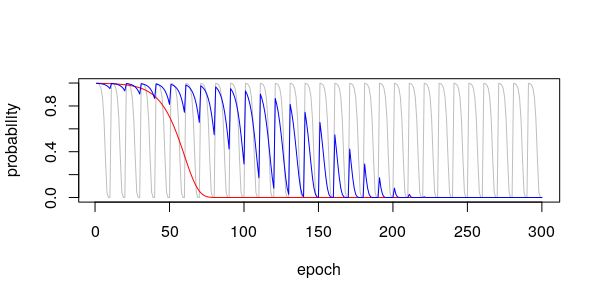
\includegraphics[width=\textwidth]{./graphics/sa_prob.png}
    \caption{Probability of accepting a nonimproving solution for simulated annealing metaheuristics. Three colours show three tested scenarios of cooling schedule. Red line shows slower cooling schedule, which was lead only by current iteration. Remaining scenarios involved the change of tested data per \textit{epoch}. Blue curve illustrates the best-observed scenario.}
\label{fig:sa-cooling-scenarios}
\end{figure}

\subsection{Guided local search}
\label{subsec:res-ss-gls}

Guided local search can escape local optima by the change of the evaluation method. Our goal was set to escape not local optima, but unwanted solutions with fitness equal to 0, which we refer as \textit{connection bug}. We penalise \textit{unconnected} solutions by the number of connectors. The densely connected individuals have higher fitness than sparse individuals. This penalisation proved to lead to more connected solutions faster.

\todo{Petr's comment: sem pridat ifno, ze je to bezna praxe - nejprev se optimalizuje na vykon, pak na usporu (se zachovanim vykonu)}

\todo{move table:res-usable-gls here?}

In contrast, solutions with fitness higher than 0.9 are penalised, if they have too many connectors. We expected that the circuit of strong distinguisher would be sparser, which was also verified by the experiments. The both penalization methods were tested independently, and they both have a similar role in the improvement of the results of \textit{benchmarking functions}. However, they are working especially well together, as they hold the circuits reasonable dense.

The penalisation for increasing connectivity can be referred as \textit{space exploration}, while the penalisation for reducing connectivity corresponds to \textit{solution exploitation}, concepts well known from machine learning. For further explanation, please refer to Talbi~\cite[section 1.3.3, page 24]{talbi2009metaheuristics}.

\subsubsection{\textbf{Analysis of resulting circuit}}
\label{subsubsec:res-ss-gls-circ-anal}

EACirc in this setup outperforms all other tested methods. However, we had also set a secondary goal of this approach, which is a simplification of the output circuit.

For this analysis, we had to prepare visualisation of the output circuit. The EACirc dumps the final circuit to a file in \texttt{dot} language, which is transformed to image via Graphviz visualisation tool~\cite{ellson2001graphviz}.

We also perform \textit{pruning} of the circuit, which removes unnecessary connectors and nodes. It is implemented BFS traversal of the circuit from the output node. This way, we can remove all connectors and nodes, which are not affecting the output. The \textit{pruning} works better for sparse circuits, where it can reduce the number of connectors by more than 50\,\%. Dense circuits can sometimes be pruned by less than 10\,\%.

The output from a run using Guided local search created a significantly sparser circuit, usually already with less than 50\,\% of connectors of Iterative local search runs, as is shown in~\cref{fig:ils-circuits,fig:gls-circuits}. The \textit{pruning} of such circuits resulted in very sparse circuits in overall 20 runs. These simpler circuits are easier for analysis, and they reveal additional information about the tested function. The \textit{pruning} is an important tool for manual cryptanalysis. The cryptanalysts can reveal potential weaknesses of the cryptographic function based on a simple circuit. The visualisation and pruning also help our team with understating the EACirc computations.

Pruning works only for individuals that are good distinguishers. If the tested data seem random, guided local search would not create sparse circuit -- it will remain even more connected. The density of the circuit can also show, how successful distinguisher it is.


\begin{figure}
\begin{changemargin}{-3cm}{-3cm}
\centering
\begin{subfigure}{.6\textwidth}
  \centering
  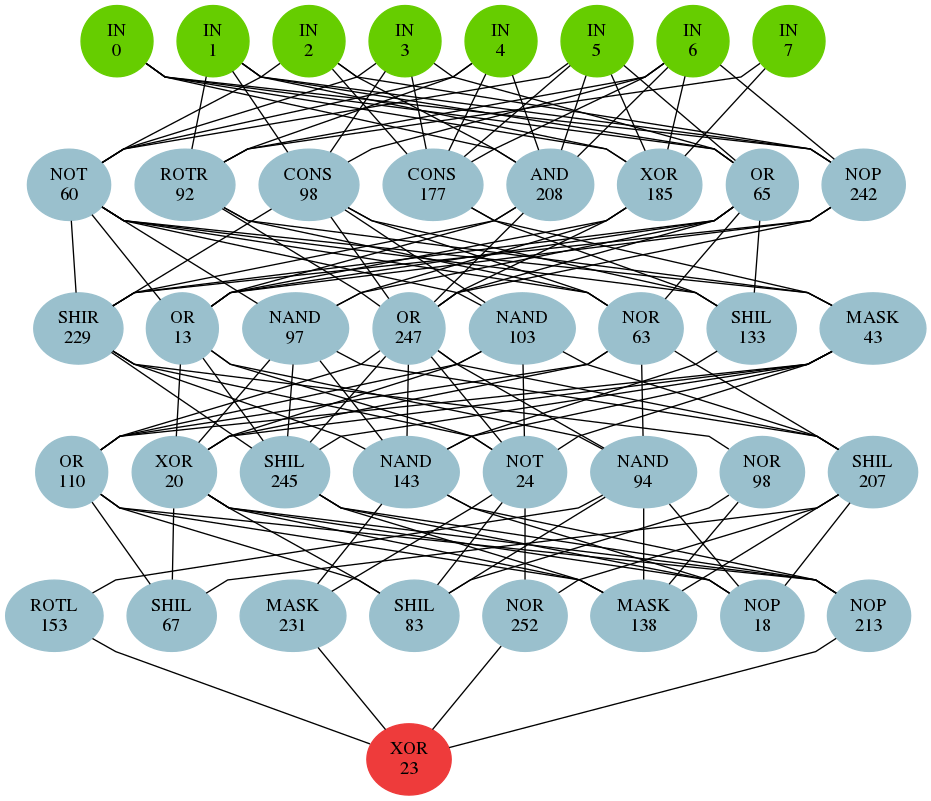
\includegraphics[width=.98\textwidth]{./graphics/ils/circuit.png}
  \caption{Circuit before pruning}
  \label{fig:ils-circuit-unpruned}
\end{subfigure}% % this comment has to be here
\begin{subfigure}{.6\textwidth}
  \centering
  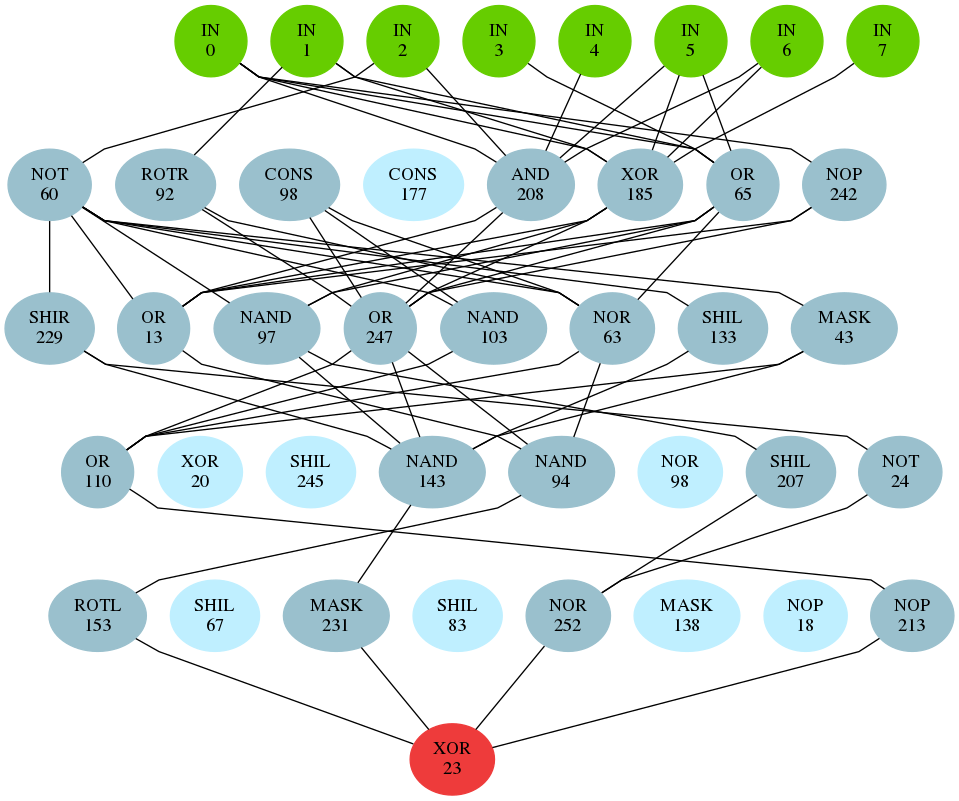
\includegraphics[width=.98\textwidth]{./graphics/ils/pruned.png}
  \caption{Circuit after pruning}
  \label{fig:ils-circuit-pruned}
\end{subfigure}
\end{changemargin}
\caption{An average solution by iterated local search for AES reduced to two rounds. Both unpruned and pruned circuits are quite dense.}
\label{fig:ils-circuits}
\end{figure}

\begin{figure}
\begin{changemargin}{-3cm}{-3cm}
\centering
\begin{subfigure}{.6\textwidth}
  \centering
  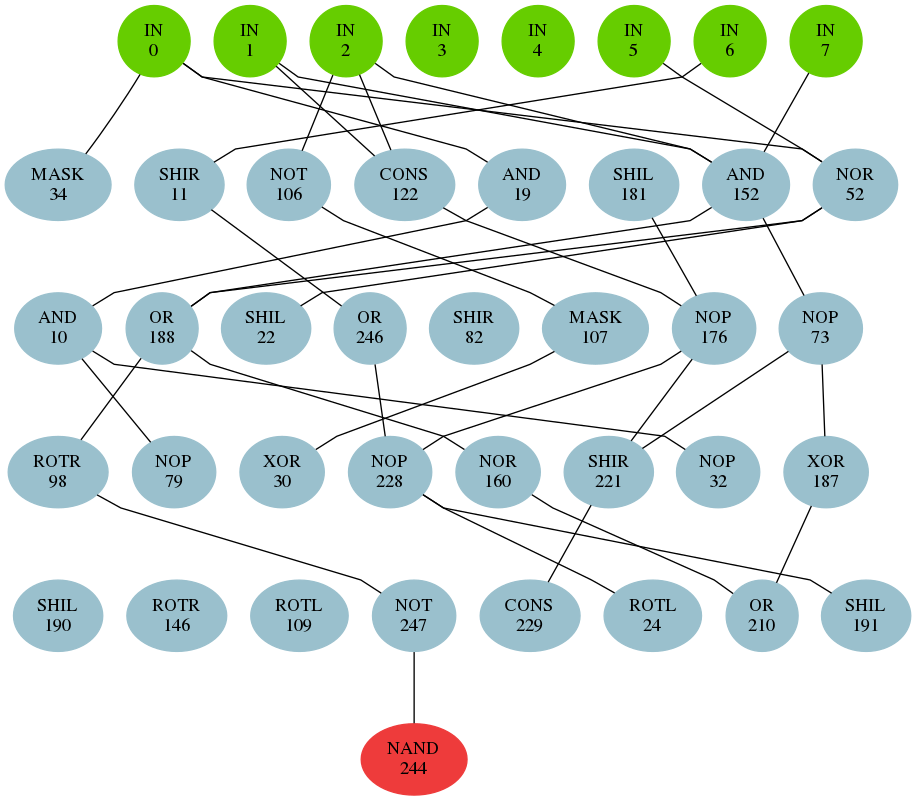
\includegraphics[width=.98\textwidth]{./graphics/gls/circuit.png}
  \caption{Circuit before pruning}
  \label{fig:gls-circuit-unpruned}
\end{subfigure}% % this comment has to be here
\begin{subfigure}{.6\textwidth}
  \centering
  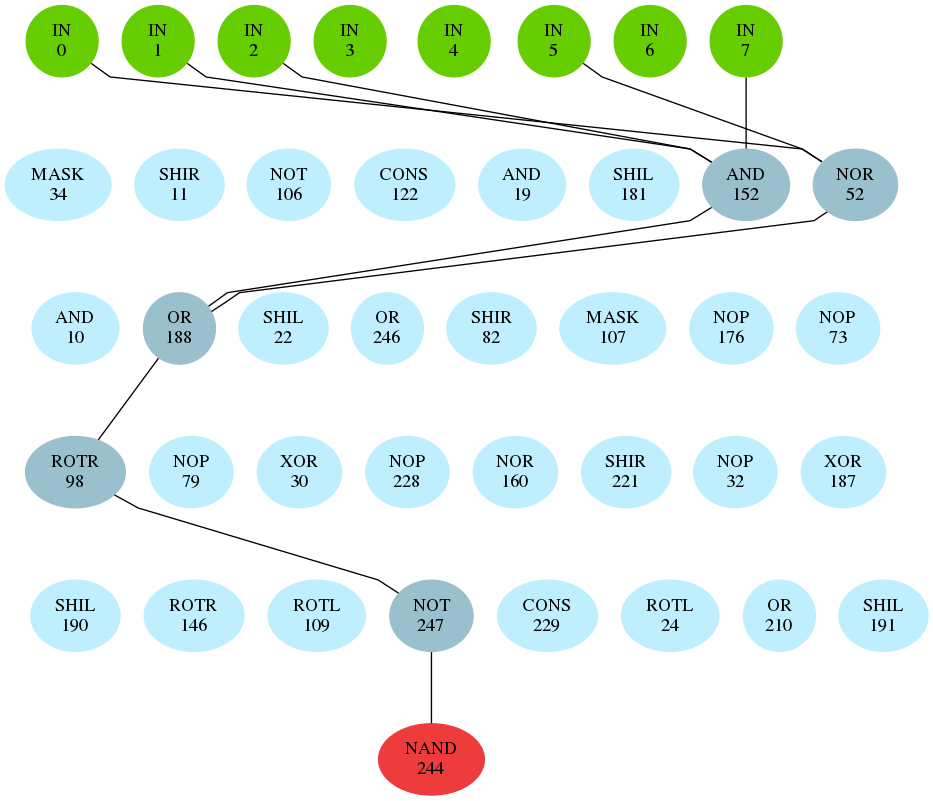
\includegraphics[width=.98\textwidth]{./graphics/gls/pruned.png}
  \caption{Circuit after pruning}
  \label{fig:gls-circuit-pruned}
\end{subfigure}
\end{changemargin}
\caption{An average solution by guided local search for AES reduced to two rounds. Even unpruned circuit is much sparser than pruned circuit from iteratel local search. However, if the solution is not performing well (we cannot find distinguisher), the circuit would be even denser than \cref{fig:ils-circuit-unpruned}.}
\label{fig:gls-circuits}
\end{figure}

\subsubsection{\textbf{Unrelated fitness functions}}

We have also analysed the original idea of Guided local search, such that we should change between unrelated fitnesses to help the metaheuristic to find a better solution. We implemented another fitness method called \textit{weight evaluator}, which do not use the $\chi^{2}$ test. The output of the circuit is evaluated bit-by-bit as a guess about the source of the tested vector. These guesses are sum per all random test vectors and all test vectors from the tested function. For 1\,000 test vectors per each dataset and one output byte, this means 8\,000 guesses per dataset. Random guesses should have a similar amount of zeroes and ones within datasets-to-dataset. The dataset-to-dataset difference in for example number of ones is described by binomial distribution with same probability $p = 0.5$ and $N = 8\,000$. We know this expected distribution of the guesses; therefore we can compute the $p$-value of the measured data, and the $p$-value is used as a fitness function. Our analysis of this separate fitness function showed it is performing slightly worse than the $\chi^{2}$ test, as it tests only one criterion of the output, while the $\chi^{2}$ test can also detect other statistical sources of nonrandomness.

Concurrent usage of those both fitnesses resulted in significantly worse distinguishing capabilities than the first method described in this sub-section. For example, this approach was not able to distinguish three round AES.


\subsection{Variable neighbourhood search}
\label{subsec:res-ss-vns}

The goals of the variable neighbourhood search are very similar to guided local search. We would also like to increase density in case of unconnected circuits and decrease the density, if the circuit works as a good distinguisher. The guided local search ensure this trough changes of the fitness function, while variable neighbourhood search changes inspected individuals. If the circuit is not connected, it tries only denser circuits. If the circuit is working well, it considers only sparser circuits for the neighbours.

If we have an unconnected circuit, we try up to ten times addition of new connector until we do not have connected graph, which was intended to speed-up the circuit connecting process. In the opposite case, when we have a good working individual, we examine only solutions with fewer connectors.

The variable neighbourhood search is performing better than the iterative local search. However, overall it performs slightly worse than guided local search, as can be seen in the end of this chapter in inter-approach comparison in \cref{table:ss-comparison}. It is probable that the limitation of the neighbourhood does not allow exploration of a significantly better solution in case of well-working solutions.

\subsubsection{\textbf{Analysis of resulting circuit}}
\label{subsubsec:res-ss-vns-circ-anal}

Same as in \cref{subsubsec:res-ss-gls-circ-anal}, we inspected the density of the output circuit. Again, the circuits were on average sparser than circuits from iterated local search. However, they were significantly denser than circuits from guided local search runs. The observation may also support the hypothesis that limiting the neighbourhood is too strict, and disallow valuable changes in the learning process.

%\section{Multi-solutions metaheuristics}
%\label{sec:res-ms}
%\subsection{Bruteforce baseline}
%\label{subsec:res-ms-bruteforce}
%\subsection{Evolutionary algorithms}
%\label{subsec:res-ms-aco}

\section{Artificial neural networks}
\label{sec:res-ann}

We tested neural networks on the same dataset. The algorithm takes two binary files as an input -- tested data and referential random data. The first step is encoding the data to \texttt{NumPy} array of \texttt{floats}. Then we form two mutually exclusive datasets, learning and testing dataset. Both contains randomly chosen test vectors from either of the input files, together with the label of the data source.

We implemented the neural network in Python library Keras~\cite{chollet2015keras}, which is a high-level API for TensorFlow library~\cite{abadi2016tensorflow}. Keras allows simple prototyping of network layout, while TensorFlow is a highly effective implementation of linear algebra for neural networks capable of computation on CPU and GPU.

\todo{cite the EANet.}

The network layout is showed in \cref{fig:ann-layout}. We tested many layouts and all available activation functions in Keras. The observations are following.

\begin{itemize}
    \item The network with two hidden layers performs the best, as it is capable of all the obtained results, and it is learning significantly faster both in the number of \textit{epochs} and in the computational time.
    \item The best activation functions are \textit{sigmoid} and its approximations \textit{tanh} and \textit{softsign}. The activation functions correspond to the bit encoding, probably different encoding of the test vectors would need different activation function.
    \item The amount of learning data for each \textit{epoch} is a very important parameter for fine-tuning. It was surprising, but the neural network prefers a few test vectors in more iterations. The size of the dataset differs from EACirc's behaviour. The best setup consumed only 25 test vectors per epoch, while the whole computation consisted of 100 epochs and the total computational time was below 30 seconds on four cores CPU. It means that the neural network can be a very naïve statistical test of randomness using only 40\,kB of analysed data. \todo{Petr: je opravdu prekvapive? Jak vypada zakladni literatura na toto tema? Answer: literature "the more data, the beter". We "the less data in one iteration, the better + increase number of epochs"}
\end{itemize}

\begin{figure}[H]
\begin{changemargin}{-\lmar}{-\rmar}
\centering{}

% Declare layers
\pgfdeclarelayer{background}
\pgfsetlayers{background,main}

\scalebox{0.77}{
\begin{tikzpicture}[scale=.8,cap=round]
    % positions
    \def \firstLayer {10}
    \def \secondLayer {8}
    \def \thirdLayer {6}
    \def \fourthLayer {4}

    % brackets
    \draw [decorate,decoration={brace,amplitude=10pt},xshift=-4pt,yshift=0pt]
(-0.2,\firstLayer - 0.8) -- (-0.2,\firstLayer + 0.8) node [black,midway,xshift=-1.2cm] 
{\footnotesize \textit{Input layer}};

    \draw [decorate,decoration={brace,amplitude=10pt},xshift=-4pt,yshift=0pt]
(-0.2,\thirdLayer - 0.5) -- (-0.2,\secondLayer + 0.5) node [black,midway,xshift=-1.4cm] 
{\footnotesize \textit{Hidden layers}};

    \draw [decorate,decoration={brace,amplitude=10pt},xshift=-4pt,yshift=0pt]
(-0.2,\fourthLayer - 0.8) -- (-0.2,\fourthLayer + 0.8) node [black,midway,xshift=-1.3cm] 
{\footnotesize \textit{Output node}};

    \draw [decorate,decoration={brace,amplitude=10pt},xshift=-4pt,yshift=0pt]
(0,\firstLayer + 1) -- (3,\firstLayer + 1) node [black,midway,yshift=0.6cm] 
{\footnotesize \textit{8 bits}};

    \draw [decorate,decoration={brace,amplitude=10pt},xshift=-4pt,yshift=0pt]
(14,\firstLayer + 1) -- (17,\firstLayer + 1) node [black,midway,yshift=0.6cm] 
{\footnotesize \textit{8 bits}};

    \draw [decorate,decoration={brace,amplitude=10pt},xshift=-4pt,yshift=0pt]
(8.64,\fourthLayer - 1) -- (0,\fourthLayer - 1) node [black,midway,yshift=-0.6cm] 
{\footnotesize \textit{ANN}};

    \draw [decorate,decoration={brace,amplitude=10pt},xshift=-4pt,yshift=0pt]
(17,\fourthLayer - 1) -- (8.64,\fourthLayer - 1) node [black,midway,yshift=-0.6cm] 
{\footnotesize \textit{CNN}};

    % layers
    \def \y {\firstLayer}
    \foreach \x in {0, 4, 10, 14} {
        \filldraw[fill=white] (\x,\y) circle (0.1);
        \filldraw[fill=white] (1+\x,\y) circle (0.1);
        \node at (2 + \x, \y) {$\dots$};
        \filldraw[fill=white] (3+\x,\y) circle (0.1);
    }

    
    \node at (8.5, \y) {$\dots$};
    
    \def \y {\secondLayer}
    \foreach \x in {1.5, 5.5, 11.5, 15.5} {
        \filldraw[fill=white] (\x,\y) circle (0.1);
    }

    \def \y {\thirdLayer}
    \foreach \x in {1.5, 5.5, 11.5, 15.5} {
        \filldraw[fill=white] (\x,\y) circle (0.1);
    }
    
    \filldraw[fill=white] (8.5,\fourthLayer) circle (0.1);


    %% The lines connecting the nodes are drawn in the background layer.
    %% This way we can hide the lines behind the nodes and don't worry
    %% about the width of each node.    
    \begin{pgfonlayer}{background}
        
        % ANN full furst layer
        \foreach \xa in {0, 4}
            \foreach \xb in {1.5, 5.5} {
                \draw[thin, -latex] (\xa,\firstLayer) -- (\xb,\secondLayer);
                \draw[thin, -latex] (\xa+1,\firstLayer) -- (\xb,\secondLayer);
                \draw[thin, -latex] (\xa+3,\firstLayer) -- (\xb,\secondLayer);
        }
        
        \foreach \xa in {10}
            \foreach \xb in {11.5} {
                \draw[thin, -latex] (\xa,\firstLayer) -- (\xb,\secondLayer);
                \draw[thin, -latex] (\xa+1,\firstLayer) -- (\xb,\secondLayer);
                \draw[thin, -latex] (\xa+3,\firstLayer) -- (\xb,\secondLayer);
            }
        \foreach \xa in {14}
            \foreach \xb in {15.5} {
                \draw[thin, -latex] (\xa,\firstLayer) -- (\xb,\secondLayer);
                \draw[thin, -latex] (\xa+1,\firstLayer) -- (\xb,\secondLayer);
                \draw[thin, -latex] (\xa+3,\firstLayer) -- (\xb,\secondLayer);
            }
        \foreach \xa in {1.5, 5.5, 11.5, 15.5}
            \foreach \xb in {1.5, 5.5, 11.5, 15.5} {
                \draw[thin, -latex] (\xa,\secondLayer) -- (\xb,\thirdLayer);
        }
        \foreach \xa in {1.5, 5.5, 11.5, 15.5}
            \foreach \xb in {8.5} {
                \draw[thin, -latex] (\xa,\thirdLayer) -- (\xb,\fourthLayer);
        }
        
        \draw[densely dotted] (8.5,\firstLayer+1) -- (8.5,\fourthLayer-1);
    \end{pgfonlayer}
\end{tikzpicture}
}
\end{changemargin}
\caption{The layout of neural network used for data classification. The left part is traditional neural network (\textit{ANN}) with fully connected first layer to the input, on the right is one dimensional convolution neural network (\textit{CNN}), where is the first layer connected only to one particular byte of the input.}
\label{fig:ann-layout}
\end{figure}

As the \cref{fig:ann-layout} shows, we experimented with a basic neural network and with a convoluted variant. The convoluted neural network works excellent for image and signal processing, as the convoluted layer detects local patterns. However, cryptographic functions should meet strict avalanche criterion that should suppress any data locality. A usage of CNN can be taken as a specific test for locality-specific patterns. If the reduced cryptographic function meets the strict avalanche criterion, the CNN sould perform worse, as the first layer of CNN has lower capabilities than a fully connected layer of ANN.

We also implemented specific strict avalanche criterion for two dimensional CNN into the generator. We start with a random plaintext, and we generate all plaintext with the Hamming distance one from the original plaintext. These encrypted plaintexts may share two-dimensional patterns.

Overall, the CNN performed worse than ANN. The problems were slower learning (probably due to \textit{dropout}, that is suggested to use with CNN), but sometimes the distinguisher was not found even during more epochs. The best results of ANN are summarised in the \cref{table:res-usable-ann}.

\begin{table}[H]
\centering
\begin{tabular}{l|l l l l}
Function\textbackslash{}rounds & -1 & 0 & 1 & 2\\ \hline
rnd\_rnd$_{\textnormal{no rounds}}$& -- & \fn{}0.511 & --         & --         \\\\
AES$_{3}$        & \fd{}1.0   & \fn{}0.494 & \fn{}0.482 & \fn{}0.489 \\
BLAKE$_{1}$      & \fd{}1.0   & \fn{}0.492 & \fn{}0.495 & \fn{}0.500 \\
Grain$_{2}$      & \fd{}0.999 & \fd{}1.0   & \fn{}0.492 & \fn{}0.500 \\
Grostl$_{2}$     & \fn{}0.507 & \fn{}0.504 & \fn{}0.499 & \fn{}0.506 \\
HC-128$_{0}$     & \fd{}--    & \fn{}0.014 & \fn{}0.016 & \fn{}--    \\
JH$_{6}$         & \fd{}0.999 & \fd{}1.0   & \fn{}0.512 & \fn{}0.504 \\
Keccak$_{3}$     & \fd{}0.996 & \fn{}0.504 & \fn{}0.490 & \fn{}0.498 \\
MD6$_{8}$        & \fd{}0.812 & \fd{}0.533 & \fn{}0.484 & \fn{}0.506 \\
Rabbit$_{0}$     & \fd{}--    & \fn{}0.019 & \fn{}0.007 & \fn{}--    \\
RC4$_{\textnormal{no rounds}}$& --         & \fn{}0.511 & --         & --         \\
Salsa20$_{2}$    & \fd{}0.694 & \fd{}0.663 & \fn{}0.492 & \fn{}0.508 \\
SINGLE-DES$_{4}$ & \fd{}0.512 & \fn{}0.494 & \fn{}0.492 & \fn{}0.512 \\
Skein$_{3}$      & \fd{}1.0   & \fd{}1.0   & \fn{}0.014 & \fn{}0.01  \\
SOSEMANUK$_{0}$  & \fd{}--    & \fn{}0.011 & \fn{}0.013 & \fn{}--    \\
TEA$_{3}$        & \fd{}0.980 & \fd{}0.548 & \fn{}0.500 & \fn{}0.495 \\
TRIPLE-DES$_{2}$ & \fd{}0.997 & \fd{}0.522 & \fn{}0.493 & \fn{}0.507
\end{tabular}
\caption{The best obtained results of ANN on usable testbed. The values are corresponding to \textit{acceptance rate}, where value $0.5$ is the reference value.}
\label{table:res-usable-ann}
\end{table}

An analysis of ANN learning can be evaluated by following two variables.

\begin{description}
    \item[Acceptance rate] is equal to ratio of $\frac{\#_{\textnormal{correct quesses}}}{\#_{\textnormal{total quesses}}}$. So it measures the quality of the ANN, similarly as fitness function was the metaheuristics' metric.
    \item[Crossentropy loss] describes how big changes can the network do for learning itself (similar to the temperature of simulated annealing).
\end{description}

Those values are shown for AES in 1 to 3 rounds with both ANN and CNN for comparison in \cref{fig:ann-learning}.


\begin{figure}[H]
\begin{changemargin}{-3cm}{-3cm}
\centering
\begin{subfigure}{.6\textwidth}
  \centering
  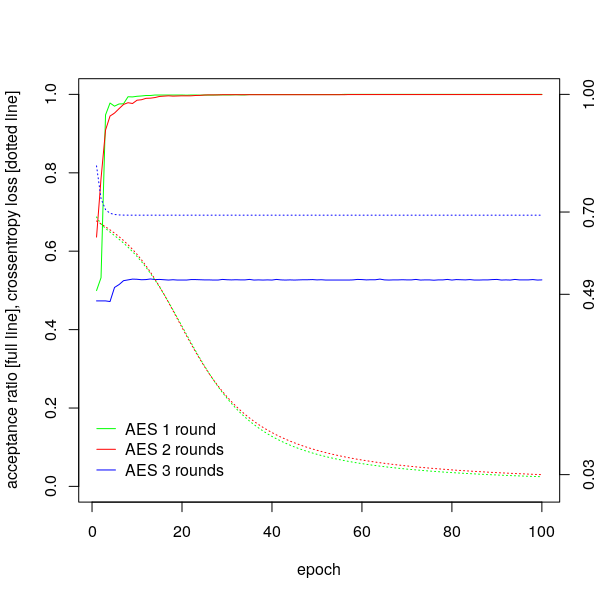
\includegraphics[width=.98\textwidth]{./graphics/ann/ann.png}
  \label{fig:ann-learning-ann}
\end{subfigure}% % this comment has to be here
\begin{subfigure}{.6\textwidth}
  \centering
  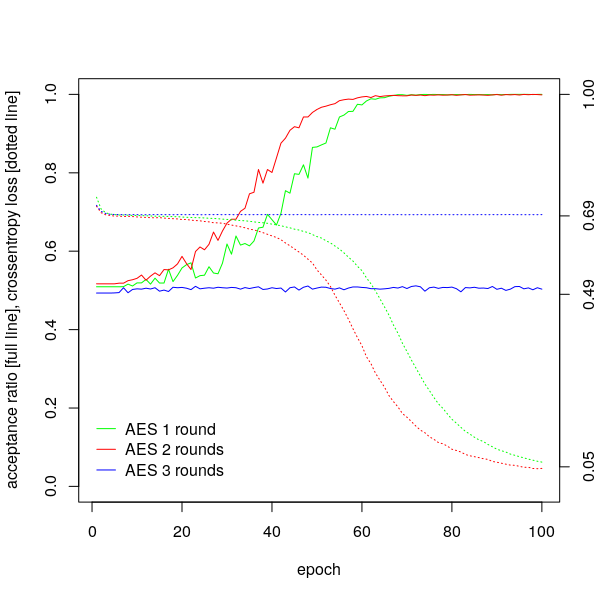
\includegraphics[width=.98\textwidth]{./graphics/ann/cnn.png}
  \label{fig:ann-learning-cnn}
\end{subfigure}
\end{changemargin}
\caption{Learning process of ANN (left) and CNN (right) on AES reduced to one to three rounds.}
\label{fig:ann-learning}
\end{figure}

\todo{Petr: dal bych do separatni podkapitoly - je neco uplne jineho nez predchozi experimenty}
We contacted pattern recognition team from University Ca’ Foscari Venice. We presented them our approach and results, and they suggested us using CNN. They also tried their own methods on the data, provided by the \textit{generator}. The results of this cooperation are still open. \todo{is this true before submition?}

% Implementation
%   preprocessing of input data
%       usage - learning data, testing data are separated
%   Keras library
% activation function
% ANN
% CNN
% automation
% intepretation
% results
% cooperation with Italy
% future work: learn on AES r2, re-learn on aes r3


%\section{Optimisation by grain fine-tuning selected metaheuristic}
%\label{sec:res-finetuning}

%% needs revision
%Trying multiple metaheuristic is broad approach. However, as stated in no free lunch theorem, there is a tendency, than no single metaheuristic guarantee better results, while dedicated human work on analysing and fine-tuning the method can bring better results.

%In~\cite{kubicek2016new}, we analysed deeply one single function -- Tiny Encryption Algorithm (\textit{TEA}). The aim of this analysis was finding best setup specific to tested function, so we can directly compare EACirc to other teams that were using genetics algorithm for testing randomness of TEA ciphertext.

%Instead of broad analysis, we tried multiple settings mainly of the tested data. The best distinguishers were found for testing strict avalanche criterion. We also tested many other constants that specify the computation.

%Intiialy, we observed worse results along all metaheuristics for TEA than are stated in the paper. Therefore, we analysed the the source of different behaviour. Due to this analysis, we found an implementation bug in EACirc 4 \todo{cite commit} that actively decreased the used size of the circuit by two layers. \todo{Updated results, other results were intouched?}.

%This unintentional analysis showed that fine-tuning the dimensions of the circuit is crucial for observing the best performance. % TODO: false!

\section{Inter-approach comparison}
\label{sec:res-comp}

The interesting details about single-solution metaheuristics are abridged in \cref{table:ss-comparison}. Both approaches of artificial neural networks are not able to distinguish data from function reduced to given number of rounds, except eight rounds MD6.

\begin{table}
\centering
\begin{tabular}{l|l l l l l}
Metaheuristic\textbackslash{}Function\_rounds   & AES$_3$ & BLAKE$_1$& MD6$_8$& DES$_5$& TEA$_4$\\ \hline
Iterative local search                          & 0.160   & 0.110    & 0.774  & 0.204  & 0.444  \\
Simulated annealing                             & \textbf{0.305} & 0.051    & 0.419  & 0.093  & 0.244  \\
Guided local search                             & 0.164   & \textbf{0.260}    & \textbf{0.995}  & \textbf{0.496}  & 0.729  \\
Variable neighbourhood search                   & 0.182   & 0.157    & 0.992  & 0.441  & \textbf{0.877}
\end{tabular}
\caption{Selected results of EACirc utilising different single-solution metaheuristics.}
\label{table:ss-comparison}
\end{table}


\begin{itemize}
    \item Guided local search is always more successful than iterated local search, and it is almost always the best among the methods. The single better result of simulated annealing does not mean it is better than guided local search, due to worse reference value because of the \textit{connection bug}. Same for better result for four rounds TEA of variable neighbourhood search, which is traded of for a longer computation time.
    \item ANN can take advantage of bit-oriented evaluation, but we have not seen any benefits of it, even though it is a crucial capability for cryptographic data
    \item Advantage of single-solution over multi-solution metaheuristics is much simpler interpretation, as we do not care about the dependency of the statistic result.
    \item The runtime of simulated annealing and guided local search is same as runtime of iterated local search. The variable neighbourhood search can take up to five times longer. The data consumption of all metaheuristics in EACirc is the same, described in \cref{fig:dataUsage}.
    
    In comparison, the neural networks need significantly less data (as was shown in \cref{fig:ann-dataUsage}). One run of ANN takes about ten times shorter as one run of EACirc. However, due to varying capabilities, these numbers are not comparable. EACirc can find distinguisher for AES reduced to two rounds within less than ten epochs, compared to common 300. Interesting comparison of the efficiency of EACirc implementation is that \texttt{C++} EACirc consumes twelve times more data per second of computation than ANN implemented in \texttt{Python}.
    
    Still, the ANN is the only method, can can be used to classify a single test vector (like 16 bytes). The framework provides both its classification guess and the estimation of its certainty in the guess. No other method provides such application.
\end{itemize}

\chapter{Related work}
\label{chap:relatwork}

We presented our tools for randomness assessment, yet this area is broad, and many researchers developed their own tools. Most commonly, the tools are not adaptive to the data. Instead, they test the data for a set of statistical properties. These statistical tests are grouped to statistical test batteries. There are multiple batteries, we present the followings.

%Assesment of randomness is necessary in other fields than just cryptography. Physicists use randomness assesment for .... Overal, all research areas need to evaluate their data by statisticaal tests. Therefore, statistical testing is well studied field with multiple standard tools. There are multiple statistical batteries. 

\begin{description}
    \item[Donald Knuth] explains statistical testing in the second edition of The Art of Computer Programming~\cite{knuth1969vol}. He suggested several PRNGs, and for analysis, he designed some statistical tests. The high quality of this source discouraged other researchers from work in this area until George Marsaglia came with the Diehard battery. \todo{cite discouraged} %zeroth
    \item[Diehard] was developed at Florida State University by George Marsaglia in 1995~\cite{marsaglia1996diehard}. It was published on CD together with three so-called true random data sources and multiple PRNGs. %first
    \item[Crypt-X suite] was a test battery for analysis of cryptoprimitives used in the late nineties~\cite{cryptxs}. NIST STS fully surpassed it. % second
    \item[NIST STS] is the golden standard of statistical testing in cryptography~\cite{rukhin2001statistical}. NIST standardised part of the battery as one step for certification FIPS 140-1 and more strict FIPS 140-2. It was also used as one criterion of evaluation of AES candidates, evaluated by Murphy in~\cite{murphy2000power}. For example, Murphy found that the AES candidate HPC failed in NIST STS, which detected possible weaknesses of the algorithm.

    NIST STS was developed in the late nineties, and the last revision was released in 2010~\cite{rukhin2001statistical}. The 2010 update removed biased test \textit{Lempel-Ziv Complexity of Sequences}. Further analysis of the bias in the $p$-values produced by NIST STS shows more dependent tests, which leads to a production of biased results. Overall NIST STS is accepted as a "golden" standard, so newer batteries extend it (at least the FIPS 140 subset of NIST STS battery) and relates to it. % third
    \item[Dieharder] was developed by Robert G. Brown at the Duke University in 2004~\cite{brown2013dieharder}. It reimplements all tests of Diehard battery, and extends it by many additional tests. Dieharder also contains three of fifteen test of NIST STS battery. However, it suffers similar bias flaws as NIST STS, as detected \todo{Lubo in}. % fourth
    \item[TestU01] is state of the art in statistical testing. It is a library, continuously developed by Université de Montréal since 2007~\cite{l2007testu01}. The design of the test is innovative in comparison to previous batteries. It uses fewer tests, whose are parametrised to form more subtests. This approach outperforms all other statistical batteries, as will be shown in our results in \cref{table:res-batteries}. The TestU01 also implements multiple PRNG from different categories. % fifth
    \item[PractRand] is another competitor to TestU01~\cite{dotypractically}. The author claims PracRand suits better for testing a large amount of data in comparison to other batteries. However, we have not testified this claim.
    \item[RaBiGeTe] is user friendly battery for Windows users~\cite{rabigete}. It implements some of the NIST STS's tests and some of Donald Knuth's tests.
\end{description}

There are also others statistical batteries: CryptoStat~\cite{kaminsky2013cryptostat}, YAARX~\cite{biryukov2014automatic}, ENT, SPRNG, gjrand and BSI test suite. \todo{Petr: proc vsechny necitujes? Proc o nich neni neco uvedeno? }

% randomness is analysed in more research areas
%   statistical batteries
%       find use-cases
%       papers on stat bat in crypto (paper of NIST STS for AES competition)
% more papers on randomness analysis (in crypto) // take inspiration in TEA paper

\section{Statistical batteries}
\label{sec:relatwork-stat}

% what they are
% methodics

We evaluated the dataset of well-known functions with NIST STS (faster implementation by Sýs et al. was used~\cite{sys2016algorithm}), Dieharder and TestU01 battery. Those batteries were automated in the project Randomness testing toolkit (RTT)~\cite{rttgit} as part of the master thesis of Lubomír Obrátil~\cite{obratilMgrThesis}. RTT is online service, which allows the user to upload binary data and it executes the batteries on them. It automatically detects the best possible setting of the batteries, as they are parametrised mainly by the size of the binary file. After the execution, RTT postprocess the results and outputs human readable interpretation of them. Same as the visualisation in this thesis, it uses colours to simplify the interpretation, where red stands for rejected test and green for passed test.

Such interpretation is straightforward. However, we show it may be incorrect in a very specific situation due to statistical properties of the batteries. To prove that, we need to explain the interpretation in a statistical manner.

A single test assesses the data against the null hypothesis that the data are random. The test may reject the hypothesis and therefore state the data seems nonrandom, or it may accept the hypothesis, where it means the test cannot find enough evidence for nonrandomness of the data. However, the test may fail with an error of two types.

\begin{description}
    \item[Type I error] describes the likelihood of acceptance null hypothesis when it is false (false positive). The test incorrectly states that the data are not random. This error occurs with the probability specified by critical value $\alpha$ for random data.
    \item[Type II error] describes the likelihood of rejection null hypothesis when it is true (false negative). The test did not spot nonrandomness of the data. The probability of type II error is also dependent on $\alpha$, and its calculation is denoted $\beta$.
\end{description}

The batteries consist of a set of tests, that are parametrised up to hundreds of sub-tests. If the critical value $\alpha$ is, for example, $1\,\%$, then the probability that all 100 tests will correctly pass is $0.99^{100}=36.6\,\%$ (suppose the tests are independent, which however do not hold for sub-tests). Therefore, we have to expect type I errors. The probability of type I error further increases if the tests are dependent. Sýs et al.~\cite{sys2015interpretation} showed that some of the NIST STS tests are dependent and they proposed the interpretation of the battery based on calculated proportion of failed tests. Same authors plan to revise also Dieharder battery, which contains similar ambiguity in interpretation. Part of these results are going to be published in thesis of Lubomír Obrátil~\cite{obratilMgrThesis}. RTT uses this approach for the interpretation.

\subsection{Statistical batteries results}
\label{subsec:relatwork-stat-res}

Visualisation of results of multiple batteries required simplification of the table. The rows of the table are functions from the methodology used for previous results. The column represents single statistical battery. The cell contains a pair of round and amount of failed sub-tests of total sub-tests. Round says, how least reduced function the battery found evidence of nonrandomness. The dash means that the battery was unable to detect nonrandomness in any reduced version of the cryptographic function.

\todo{correct the table}

\begin{table}[H]
\centering{}
\hspace*{-3cm}
\begin{tabular}{l|p{1.8cm} p{1.8cm} p{1.8cm} p{1.8cm} p{1.8cm} p{1.8cm} p{1.8cm}}
Function\textbackslash{}battery &
              Dieharder & NIST STS  & TestU01 Alphabit  & TestU01 Block Alphabit    & TestU01 Crush & TestU01 Rabbit    & TestU01 Small Crush   \\ \hline
AES         & 3, 50/110 & 3, 177/188& 3, 15/33          & 3, 114/198                & 3, 94/186     & 3, 16/58          & 3, 5/15               \\
BLAKE       & 1, 17/110 & 0, 162/162& 1, 8/33           & 1, 74/198                 & 1, 86/166     & 1, 15/58          & 1, 5/15               \\
Grain       & 2, 110/110& 2, 187/188& 2, 33/33          & 2, 198/198 *              & 6, 10/186     & 2, 54/57          & 2, 14/14              \\
Grostl      & 2, 70/110 & 2, 182/188& 2, 27/33          & 2, 152/198                & 2, 134/186    & 2, 27/58          & 2, 9/15               \\
HC-128      & --        & --        & --                & --                        & --            & --                & --                    \\
JH          & 6, 110/110& 6, 161/162& 6, 33/33          & 6, 196/198                & 6, 153/169    & 6, 50/58          & 6, 15/15              \\
Keccak      & 2, 106/110& 2, 187/188& 2, 33/33          & 3, 51/198                 & 3, 39/186     & 3, 9/58           & 2, 15/15              \\
MD6         & 8, 59/110 & 8, 159/188& 8, 21/33          & 9, 11/198                 & 9, 13/186 *   & 9, 5/58           & 8, 6/16               \\
Rabbit      & --        & --        & 2, 4/33           & 3, 11/198                 & 4, 12/186 *   & 3, 5/58 *         & --                    \\
RC4         & --        & --        & --                & --                        & --            & --                & --                    \\
Salsa20     & 2, 77/110 & 2, 162/188& 2, 27/33          & 2, 155/198                & 2, 147/186    & 2, 34/58          & 2, 13/15              \\
SINGLE-DES  & 5, 38/110 & 4, 24/188 & 5, 5/33           & 5, 74/198                 & 5, 55/186     & 5, 13/58          & 4, 12/15              \\
Skein       & 3, 96/110 & 3, 162/188& 4, 5/33           & 4, 50/198                 & 4, 18/186     & 4, 8/58           & 3, 15/15              \\
SOSEMANUK   & 4, 110/110& 4, 162/162& 4, 33/33          & 4, 198/198                & 4, 163/168    & 4, 55/58          & 4, 15/15              \\
TEA         & 4, 54/110 & 4, 51/188 & 4, 17/33          & 5, 27/198                 & 5, 8/186      & 4, 22/58          & 4, 7/15               \\
TRIPLE-DES  & 3, 26/110 & 2, 162/188& 2, 32/33          & 3, 12/198                 & 3, 10/182     & 2, 52/58          & 2, 14/15              
\end{tabular}
\caption{Application of statistical batteries on data from round-reduced well-known cryptographic functions. Cell contain a pair of the highest number of rounds, to which was the cryptographic function reduced and the number of failed sub-tests per total amount of sub-tests in the battery. Note that the total quantity of sub-tests is changing. The number of sub-tests depends on the data properties, as the batteries requires some assumptions on the tested data for execution of some sub-tests. The results were computed by Randomness Testing Toolkit. Complete results with detailed information about which tests are passing can be found on \href{http://rtt.ics.muni.cz/ViewResults/?created_from=2017-04-24+12\%3A00\%3A00&created_to=2017-04-29+00\%3A00\%3A00}{RTT page (as results from 2017-04-24 to 2017-04-28)}.}
\label{table:res-batteries}
\end{table}

From those results, we have multiple observations.

\begin{itemize}
    \item EACirc performs similarly to NIST STS, Dieharder and TestU01 Small Crush.
    \item TestU01 Crush outperforms all other batteries, which is traded-of by its computation time.
    \item High amount of failed test indicates the data are biased in multiple characteristics. Such data are usually rejected by all batteries. However, when only a single battery detects nonrandomness, it is TestU01.
    \item \textbf{TestU01 was able to detect deviances in full Rabbit cipher.} After analysis of this result, we found that there was a report \textit{On a bias of Rabbit}~\cite{aumasson2007bias} during the eSTREAM competition, which discovered the same property. Even though this bias was found, Rabbit cipher was selected as hardware profile finalist, stating that the bias does not allow any feasible attack due to complexity.
    \item Similarly observation is the bias of another hardware profile eSTREAM finalist Grain. TestU01 Crush can detect bias up to six rounds Grain, which is almost one-half of the full function (13 rounds). The known \textit{dynamic cube attack} on the same version of Grain~\cite{dinur2011breaking} do not explain the bias observed by us. Our round reduction is based on a limitation of the shuffle of the non-linear feedback shift registers, which may require more than six rounds to shuffle the data enough. The full Grain cipher has 13 rounds, which still provides some security margin.
    \item The interpretation based on the probability of fail of $n$ sub-tests would not detect the nonrandomness property of Grain reduced to five rounds. The rejection approach is strict (so it has hight probability of type II error), however manual observation that the failed sub-tests are the same as failed subtests of four and six rounds Grain provide necessary trust to our interpretation that the data are biased.
    \item Note: MD6 reduced to 10 rounds is nonrandom based on TestU01 Crush and Rabbit. The results in the table were omitted due to consistency, as the interpretation method leaves them as passed test. However, the probability of those extreme results is below 1\,\%. The same behaviour was detected for RC4 by TestU01 Crush.
    \item Rejection of randomness by the battery do not have to be taken as black-box (as we present here), but we can analyse, which test failed. However, depending on the test, it may be more difficult than analysis of the output circuit from EACirc.

    EACirc may also provide concrete proof of the data dependency. If there is a dependency between specifics bytes, it would always be present in the circuit for strong distinguishers. The statistical battery would some test, probably the \textit{dependency test}. However, they would not state, what is the dependence in the data.
    \item Another advantage of EACirc is the simplicity of already learned distinguisher. Using learned distinguisher needs much less data, only low kilobytes and it may even state the guess for a single test vector. The test of statistical battery always requires fixed amount of data.
\end{itemize}

\section{Compression algorithms}
\label{sec:relatwork-compress}

One of the definitions of randomness is via Kolmogorov's complexity. Data are random if they cannot be compressed. The data from the cryptographic function can always be compressed, but the computation would require finding the key used for the encryption; therefore such compression is not feasible.

We experimented with this approach, trying capabilities of compression programs. We have analysed following Unix lossless data compression utilities.

\begin{description}
    \item[zip] is compression utility based on Deflate algorithm. It combines LZ77~\cite{ziv1977universal} and Huffman coding algorithms.
    \item[gzip] is GNU version of \textit{zip} utility.
    \item[lzop] is compression utility using LZO algorithm. It aims for faster decompression; however, the compression can be less efficient than \textit{gzip}.
    \item[bzip2] is compression algorithm based on Burrows–Wheeler transformation~\cite{burrows1994block} of the reoccurring sequences to strings of identical letters. Then it applies the move-to-front transformation and Huffman coding. 
    \item[NanoZip] in version 0.09a is the latest version from the year 2011 of an experimental archiver software based on Burrows-Wheeler compression~\cite{nanozip}. Based on multiple data compression benchmarks, NanoZip has the highest compression capabilities. Although we used various parameters, we did not obtain archive, which could be losslessly decompressed. Therefore we omit this algorithm.
\end{description}

All the utilities were executed with highest compression ratio with the slowest speed.

We denote the results in a similar manner as results of the batteries. The rows are labelled by cryptographic functions, columns are compression utilities. The cell is a pair of the round count that we executed the algorithm, and compression ratio, which says how much data we safe. Compression of random data should not safe anything, marked with dash, whatever higher means the data are nonrandom. We tested this evaluation experimentally on random data, and the compressed file was never smaller than the original file. This property was tested for more than ten samples. The dash means that the compression algorithm was unable to detect nonrandomness compress the data from any reduced version of the cryptographic function.

\begin{table}[H]
\centering{}
\begin{tabular}{l|p{1.8cm} p{1.8cm} p{1.8cm} p{1.8cm}}
Function\textbackslash{}algorithm & 
                bzip2   &   gz      &   lzop    &   zip     \\ \hline
AES         & 2, 2\,\%  & 2, 15\,\% & 2, 25\,\% & 2, 15\,\% \\
BLAKE       & 0, 0\,\%  & 0, 0\,\%  & 0, 1\,\%  & 0, 0\,\%  \\
Grain       & 2, 3\,\%  & 2, 11\,\% & 2, 25\,\% & 2, 11\,\% \\
Grostl      & 0, 0\,\%  & 0, 0\,\%  & 0, 1\,\%  & 0, 0\,\%  \\
HC-128      & --        & --        & --        & --        \\
JH          & 6, 57\,\% & 6, 59\,\% & 6, 68\,\% & 6, 59\,\% \\
Keccak      & 1, 16\,\% & 2, 99\,\% & 1, 36\,\% & 2, 99\,\% \\
MD6         & 7, 99\,\% & 7, 97\,\% & 6, 59\,\% & 7, 97\,\% \\
Rabbit      & --        & --        & --        & --        \\
RC4         & --        & --        & --        & --        \\
Salsa20     & --        & 2, 99\,\% & --        & 2, 99\,\% \\
SINGLE-DES  & 2, 71\,\% & 2, 79\,\% & 2, 84\,\% & 2, 78\,\% \\
Skein       & 2, 93\,\% & 2, 79\,\% & 2, 93\,\% & 2, 80\,\% \\
SOSEMANUK   & 4, 0\,\%  & 4, 0\,\%  & 4, 1\,\%  & 4, 0\,\%  \\
TEA         & 2, 97\,\% & 3, 99\,\% & 2, 93\,\% & 3, 99\,\% \\
TRIPLE-DES  & 2, 99\,\% & 2, 98\,\% & 2, 99\,\% & 2, 98\,\% 

\end{tabular}
\caption{Capabilities of compression algorithms on cryptographic data. Cell contain pair of highest number of rounds, to which was the cryptographic function reduced and saved space ratio of the compression.}
\label{table:res-compression}
\end{table}

Observations from the results are following.

\begin{itemize}
    \item The efficiency of newer \textit{bzip2} on cryptographic data is not higher than efficiency of \textit{gzip} and \textit{zip}.
    \item The fact that we have to reduce functions to very few rounds is probably caused by character (byte-level) specialisation of the compression algorithms. The cryptographic data may contain more bit-level dependencies.
    \item Still the compression algorithms state similarly to results of neural networks. From these results, we can assume that neural networks detected only the disproportion of zeroes and ones or simple byte-level patterns.
\end{itemize}

% Kolmogorov's information (definition of randomness)
% Specialised for detection of byte-level patterns
%   quite good for this - already long developed
% List of algorithms with links
% Results

\section{Metaheuristcs for randomness testing}
\label{sec:relatwork-paper}

Besides statistical batteries, numerous other works did the cryptanalysis based on testing some of the statistical properties. We have encountered several works using genetics for statistical analysis of cryptoprimitives. Most of them analysed Tiny Encryption Algorithm (TEA), which is a simple block cipher designed by D. Wheeler and R. Needham in 1995~\cite{TEA}. It was used as a benchmark due to its simplicity and well-known vulnerabilities~\cite{TEAAttack}. The application of genetics programming started in 2002 by J. Hernández et al.~\cite{twoRoundsTea}, whose found statistical deviance in two rounds TEA. Further improvements from the team were presented in 2004 finding the non-randomness in three and four rounds TEA as well~\cite{fourRoundsTea}. So far the best results using genetic programming were found by W. Hu~\cite{fiveRoundsTea}, who detected non-random properties for five rounds TEA. We compared EACirc with these results in~\cite{2016-infocommunications-kubicek}.

The Genetic programming was also used for analysis of four rounds DES~\cite{song2007cryptanalysis}. DES was also analysed using particle swarm metaheuristic in~\cite{shahzad2009cryptanalysis}, and Simplified DES was analysed by Simulated Annealing, and Tabu search in~\cite{nalini2005cryptanalysis}. The best so far metaheuristic cryptoanalysis on DES were on eight rounds DES using genetic programming by Husein et al.~\cite{husein2007genetic}. In general, these methods are worse than statistical batteries in the number of rounds, but they can provide additional information to the cryptanalyst that batteries do not.

% Take papers from TEA paper
% Compare with EAC and show the results and CITE our paper

\chapter{Conclusion}
\label{chap:conclusion}

\section{Summary}
\label{sec:conclusion-summary}

This work analysed the application of metaheuristics in randomness testing tools, especially in EACirc tool. The possibility of implementation with the potential issues was discussed in the \cref{chap:optimisation}. We extended EACirc tool by three new metaheuristics that represented different single-solution metaheuristics types. Guided local search metaheuristic performs better than the former algorithm. In addition, it proved to significantly simplify output distinguisher, which reduces the complexity of further cryptanalysis. Therefore will be guided local search incorporated into the following release of the EACirc tool as default metaheuristic.

Another tested method was using the artificial neural network. The results were unsatisfactory, proving no free lunch theorem. This area requires more work to achieve better results, and it may be necessary significantly redesign the neural network algorithms. The artificial neural network works with floating points, and the discrete bit-level patterns do not fit the gradient descent algorithm with analysed data representation and activation functions. As we examined the literature within this area, we have found no mature theory. It is still an open question if the artificial neural network can achieve better results in the recognition of cryptographic data. This area and tool developed in this work are continued by Italian researchers.

In comparison to state of the art in randomness testing, all out methods perform worse than the TestU01 statistical battery. In comparison with other statistical batteries, EACirc finally reached their results. The only advantage of EACirc over TestU01 is the analysis of the developed distinguisher, which may need less statistical knowledge than understanding TestU01 test and can point concrete bytes dependencies. TestU01 Crush, the strongest battery setting, found bias of full Rabbit function, which showed to be a replication of already known results discovered during eSTREAM competition.

An important product of this work is the testbed of well-known cryptographical function, which is an extension and correction of previous testing sets. Besides, we presented generator tool for the direct generation of the tested data, which can be used by developers of others randomness testing tools as a benchmark. It can be used as well by cryptographers to generate specifically modified cryptography data, usually reduced in the number of rounds.

\section{Future work}
\label{sec:conclusion-future}

With many works on EACirc, the capabilities increased to the level od Dieharder battery. I would estimate that current approach using byte-oriented circuits is unable to compete directly with the TestU01 battery. EACirc can focus more on the analysis of the circuits, which offers an addition value over the TestU01.

The another project based on polynomials shows better results as it is bit-oriented. It does not utilise any metaheuristic, hence application of multi-solution metaheuristic like evolutionary algorithms, or swarm intelligence may increase its already promising capabilities. The work on the integration of those metaheuristics already started within this thesis.

The testbed of well-known functions can be further extended by different means of reduction of the cryptographic functions RC4 and HC-128. For RC4, we can use bit selection capabilities of the generator. All functions can also take advance of currently in progress automatic customisation of functions introduced in the thesis of Radka Cieslarová~\cite{cieslarovaBcThesis}. We refer to this project as Heatmaps.

The heatmaps are one of the development plans with the generator tool. Other plans extend the tool by already implemented CAESAR functions and new PRNG. Altogether with randomness testing toolkit is planned as a publication for \todo{...}.

%\begin{itemize}
    %\item EA/ANN/swarm intelligence on polynomials + publication plan
    %\item RC4 and HC-128 cannot be round-reduced, but we can modify them in different manner to obtain biased result. We can either apply postprocessing streams to select only specific bits of the output, or we can turn of parts the cipher. The second option was analysed in thesis of Radka Cieslarová~\cite{cieslarovaBcThesis}.
    %\item ANN with Italy
    %\item It would be useful to extend the benchmarking set by more tunable function, with slowly increasing entropy
    %\item Generator publication plan
%\end{itemize}

\chapter*{Acknowledgment}
\label{chap:ack}

Computational resources were provided by the CESNET LM2015042 and the CERIT Scientific Cloud LM2015085, provided under the programme "Projects of Large Research, Development, and Innovations Infrastructures".

Computational resources were supplied by the Ministry of Education, Youth and Sports of the Czech Republic under the Projects CESNET (Project No. LM2015042) and CERIT-Scientific Cloud (Project No. LM2015085) provided within the program Projects of Large Research, Development and Innovations Infrastructures.

We also acknowledge the support of Czech Science Foundation, the project GA16-08565S.


%%bibliography
\printbibliography[heading=bibintoc] %% Print the bibliography.

\chapter*{Appendix}
\label{chap:app}

\section{Glossary}
\label{sec:app-glos}

\todo{Sort it lexicographically}

\begin{description}
    \item[Term] explanation
    \item[Generator] explanation
    \item[Connection bug] explanation
    \item[Ciritcal value $\alpha$] explanation
    \item[Benchmarking functions] explanation
    \item[Pruning] explanation
    \item[Binary weight] explanation
    \item[Weight evaluator] explanation
    \item[Epoch] explanation
    \item[Test vector] explanation
    \item[Space exploration] explanation
    \item[Solution exploitation] explanation
    \item[Activation function] explanation
    \begin{description}
        \item[Sigmoid] explanation
        \item[Softsign] explanation
    \end{description}
    \item[Artifitial neural network (ANN)] explanation
    \item[Convoluted neural netowrk (CNN)] explanation
    \item[Crossentropy loss] explanation
    \item[Strict avalanche criterion (SAC)] explanation
    \item[PRNG] explanation
    \item[TRNG] explanation
    \item[QRNG] explanation
    \item[Randomness testing toolkit (RTT)] explanation
    \item[Local optima] explanation
    \item[Fitness function] explanation (Fitness is defined for maximization problem. Therefore 0 is the worst, 1 is the best.)
    \item[Round reduced cryptographic function] explanation
    \item[] explanation
    \item[] explanation
    \item[] explanation
    \item[] explanation
\end{description}

\section{Single-solution metaheuristics results}
\label{sec:app-ss-res}

\begin{table}[H]
\centering
\begin{tabular}{l|l l l l}
Function\textbackslash{}rounds & -1 & 0 & 1 & 2\\ \hline
rnd\_rnd         & \fn{}0.01681 & --       & --         & --        \\\\
AES$_{3}$        & \fd{}1.0   & \fd{}0.164 & \fn{}0.015 & \fn{}--   \\
BLAKE$_{1}$      & \fd{}1.0   & \fd{}0.147 & \fn{}0.012 & \fn{}0.014\\
Grain$_{2}$      & \fd{}--    & \fd{}1.0   & \fn{}0.012 & \fn{}0.019\\
Grostl$_{2}$     & \fd{}--    & \fd{}1.0   & \fn{}0.015 & \fn{}0.011\\
HC-128$_{0}$     & \fd{}--    & \fn{}0.011 & \fn{}0.007 & \fn{}0.009\\
JH$_{6}$         & \fd{}--    & \fd{}1.0   & \fn{}0.017 & \fn{}0.009\\
Keccak$_{3}$     & \fd{}1.0   & \fn{}0.01  & \fn{}0.015 & \fn{}0.012\\
MD6$_{8}$        & \fd{}--    & \fd{}0.823 & \fn{}0.009 & \fn{}0.009\\
Rabbit$_{0}$     & \fd{}--    & \fn{}0.01  & \fn{}0.011 & \fn{}0.011\\
RC4$_{no~rounds}$& --         & \fn{}0.008 & --         & --        \\
Salsa20$_{2}$    & \fd{}--    & \fd{}1.0   & \fn{}0.009 & \fn{}0.009\\
SINGLE-DES$_{4}$ & \fd{}1.0   & \fd{}0.209 & \fn{}0.01  & \fn{}0.007\\
Skein$_{3}$      & \fd{}1.0   & \fd{}1.0   & \fn{}0.018 & \fn{}0.03 \\
SOSEMANUK$_{0}$  & \fd{}--    & \fn{}0.012 & \fn{}0.007 & \fn{}0.011\\
TEA$_{3}$        & \fd{}--    & \fd{}1.0   & \fn{}0.01  & \fn{}0.012\\
TRIPLE-DES$_{2}$ & \fd{}--    & \fd{}1.0   & \fn{}0.015 & \fn{}0.009
\end{tabular}
\caption{Results of simulated annealing as EACirc metaheuristics on usable testbed.}
\label{table:res-usable-sa}
\end{table}

\begin{table}[H]
\centering
\begin{tabular}{l|l l l l}
Function\textbackslash{}rounds & -1 & 0 & 1 & 2\\ \hline
rnd\_rnd         & \fn{}0.01191 & --       & --         & --        \\\\
AES$_{3}$        & \fd{}1.0   & \fd{}0.175 & \fn{}0.013 & \fn{}--   \\
BLAKE$_{1}$      & \fd{}1.0   & \fd{}0.228 & \fn{}0.011 & \fn{}0.008\\
Grain$_{2}$      & \fd{}--    & \fd{}1.0   & \fn{}0.014 & \fn{}0.01 \\
Grostl$_{2}$     & \fd{}--    & \fd{}1.0   & \fn{}0.014 & \fn{}0.018\\
HC-128$_{0}$     & \fd{}--    & \fn{}0.013 & \fn{}0.01  & \fn{}--   \\
JH$_{6}$         & \fd{}--    & \fd{}1.0   & \fn{}0.008 & \fn{}0.017\\
Keccak$_{3}$     & \fd{}1.0   & \fn{}0.013 & \fn{}0.008 & \fn{}--   \\
MD6$_{8}$        & \fd{}--    & \fd{}0.993 & \fn{}0.006 & \fn{}0.016\\
Rabbit$_{0}$     & \fd{}--    & \fn{}0.011 & \fn{}0.009 & \fn{}--   \\
RC4$_{no~rounds}$& --         & \fn{}0.013 & --         & --        \\
Salsa20$_{2}$    & \fd{}--    & \fd{}1.0   & \fn{}0.017 & \fn{}0.01 \\
SINGLE-DES$_{4}$ & \fd{}1.0   & \fd{}0.523 & \fn{}0.014 & \fn{}0.016\\
Skein$_{3}$      & \fd{}1.0   & \fd{}1.0   & \fn{}0.01  & \fn{}0.019\\
SOSEMANUK$_{0}$  & \fd{}--    & \fn{}0.007 & \fn{}0.007 & \fn{}--   \\
TEA$_{3}$        & \fd{}--    & \fd{}1.0   & \fn{}0.016 & \fn{}0.01 \\
TRIPLE-DES$_{2}$ & \fd{}--    & \fd{}1.0   & \fn{}0.012 & \fn{}0.013
\end{tabular}
\caption{Results of guided local search as EACirc metaheuristics on usable testbed.}
\label{table:res-usable-gls}
\end{table}

\begin{table}[H]
\centering
\begin{tabular}{l|l l l l}
Function\textbackslash{}rounds & -1 & 0 & 1 & 2\\ \hline
rnd\_rnd         & \fn{}0.01124 & --       & --         & --        \\\\
AES$_{3}$        & \fd{}1.0   & \fd{}0.159 & \fn{}0.014 & \fn{}--   \\
BLAKE$_{1}$      & \fd{}1.0   & \fd{}0.134 & \fn{}0.012 & \fn{}0.014\\
Grain$_{2}$      & \fd{}--    & \fd{}1.0   & \fn{}0.007 & \fn{}0.016\\
Grostl$_{2}$     & \fd{}--    & \fd{}1.0   & \fn{}0.011 & \fn{}0.007\\
HC-128$_{0}$     & \fd{}--    & \fn{}0.011 & \fn{}0.013 & \fn{}--   \\
JH$_{6}$         & \fd{}--    & \fd{}1.0   & \fn{}0.016 & \fn{}0.011\\
Keccak$_{3}$     & \fd{}1.0   & \fn{}0.015 & \fn{}0.009 & \fn{}--   \\
MD6$_{8}$        & \fd{}--    & \fd{}0.986 & \fn{}0.014 & \fn{}0.014\\
Rabbit$_{0}$     & \fd{}--    & \fn{}0.01  & \fn{}0.01  & \fn{}--   \\
RC4$_{no~rounds}$& --         & \fn{}0.01  & --         & --        \\
Salsa20$_{2}$    & \fd{}--    & \fd{}1.0   & \fn{}0.013 & \fn{}0.008\\
SINGLE-DES$_{4}$ & \fd{}1.0   & \fd{}0.428 & \fn{}0.021 & \fn{}0.008\\
Skein$_{3}$      & \fd{}1.0   & \fd{}1.0   & \fn{}0.012 & \fn{}0.011\\
SOSEMANUK$_{0}$  & \fd{}--    & \fn{}0.005 & \fn{}0.014 & \fn{}--   \\
TEA$_{3}$        & \fd{}--    & \fd{}1.0   & \fn{}0.009 & \fn{}0.013\\
TRIPLE-DES$_{2}$ & \fd{}--    & \fd{}1.0   & \fn{}0.012 & \fn{}0.011
\end{tabular}
\caption{Results of variable neighbourhood search as EACirc metaheuristics on usable testbed.}
\label{table:res-usable-vns}
\end{table}



\end{document}
